\chapter{Introduction}
The importance of computers in our everyday life has largely increased over the past few decades.
A lot of us can only hardly imagine doing their jobs without help of appropriate computer program
and we also spend a plenty of time using computers (e.g. personal computers or mobile devices) in leisure time.
The computer programs are also often used in very critical instances like autopilot in an airplane.
But the growing number of applications of computer programs brings also need for their greater safety and security.

However, guarantee of software safety and correctness is not easy task
because the programs often go through many states during computation
and it could be very time and (memory) space demanding or even impossible to check whether no undesirable thing
happens in any of those states.
One approach to ensure software quality is \emph{testing} (and dynamic analysis) which is basically based
on running a program in the different contexts and with the different inputs
and checking whether a program behavior and the outputs are the expected ones.
This method can satisfy many of the requirements for software quality and often cover the great space of the program behaviors
but on the other side it is only possible to prove presence of the errors using testing not their absence \cite{dijkstra}.
Moreover finding some errors during testing does not mean that all errors are eliminated.

The mentioned weakness of testing can be resolved by \emph{formal verification}
which is another approach to checking program correctness.
Formal verification is method for checking whether a given system meets a given specification \cite{fav:lecture}.
There are four main branches of formal verification.
The first one is \emph{model checking} which systematically explores the states of a model (e.g. model of a program) to
prove that a property holds along the whole model.
The second approach is \emph{static analysis} which is done over a source code (or some modification of it) of a system
without its explicit execution.
The third approach is \emph{abstract interpretation} where the analysis is performed by
applying abstract transformers corresponding to the original program semantics over an abstract domain.
The last one is \emph{theorem proving}.
It proves the program in standard mathematical way -- starting from axioms and proving theorems to
verify the properties of a given system.
Theorem proving could be partially automated.

This thesis deals with specific part of static analysis called \emph{shape analysis} which is focused on the verification of the programs manipulating
complex data structures (like a different kinds of lists and trees), typically allocated on the heap.
The properties checked for this class of programs are for example checking whether no dangling
pointers are dereferenced (no invalid dereference), whether all allocated memory on a heap is also freed (no memory leaks)
during the program execution or whether there is not freed pointer which has no assigned memory (no invalid free).
There are different approaches to this kind of static analysis with the different advantages.
For example, the approach based on \emph{separation logic} \cite{seplog,seplog07} provides scalability of a verification procedure.
On the other side, the automata based approach, concretely \emph{abstract tree regular model checking} (ATRMC) \cite{artmc}, is
superior in flexibility.
However, this thesis is focused on a verification procedure based on a concept of forest automata (FA) which
combines benefits of the both mentioned approaches.

Forest automata has been introduce in \cite{forester11,forester12} and they are an extension of finite automata or more precisely extension of finite tree automata (TA).
They are used as an abstract domain in related verification procedure over which a symbolic execution of a analyzed program is performed.
A prototype of this verification procedure has been implemented in a tool called \emph{Forester}.
Forester verifies programs written in C language and it can detect invalid dereferences, invalid free, memory leaks and also reachability of an error label.
It is yet able to verify non-trivial data structures like skip-list of the second and the third level
but there is still a room for its improvement.
E.g. Forester currently does not support complete C language syntax and
it is not also yet possible to check whether a found error is real or spurious.
It is also needed to refactore some parts of Forester code before extension of the tool.
A general goal of this thesis is improving Forester in the areas described further.


Since FA are highly related to the finite tree automata the first of the goals of the thesis is to implement
a version of Forester using \vata\ -- state-of-the-art library for TA manipulation \cite{libvata}.
Particularly, this consists creating an interface between Forester and VATA to employ VATA as a TA library for Forester backend
which should bring better maintainability and modularity then implement a special TA library inside Forester as it is now.
The second goal of this thesis is to design and implement \emph{backward run} for FA based verification
which enables checking spuriousness of an error found in a program.
The error could be spurious because of too high level of abstraction over FA is used.
The information gained by backward run could be used for the refinement of \emph{predicate abstraction} (one kind of abstraction over FA)
to prevent verification procedure from getting the same spurious error again.
However, Forester does not use predicate abstraction but \emph{height abstraction} now
because predicate abstraction needs the backward run.
Height abstraction is less precise and less flexible compared to predicate abstraction so implementing predicate abstraction
enables analysis of even more complex data structures like the red-black trees.
A part of the second goal is just completing and testing implementation of predicate abstraction in Forester.

The outline of this document is following.
In Chapter \ref{ch:prel} the preliminaries are given.
The verification procedure based on FA is covered in Chapter \ref{ch:fav}.
Chapter \ref{ch:tools} provides description of \vata\ and Forester tool and Chapter \ref{ch:fova} describes an implementation of the version of Forester tool using \vata.
The design of backward run for FA base verification is given in Chapter \ref{ch:backward} and its implementation is documented
in Chapter \ref{ch:impl}.
Finally,
Chapter \ref{ch:eval} contains an overview of evaluation and 
Chapter \ref{ch:concl} summarizes this master thesis.

\chapter{Preliminaries}
\label{ch:prel}

This chapter contains the definitions of the concepts further used in this thesis.
First, graphs, trees and forests are defined together along the automata accepting them in Section \ref{sec:graph}.
Then the previously defined concepts are further extended to hierarchical ones in Section \ref{sec:fah}.
This section follows the definitions and a the structure used in \cite{techrep}.

\section{Graphs, Trees and Forests}
\label{sec:graph}

Assume a word $w = a_1 \cdots a_n$, we denote $i$-th symbol of $w$ as $a_i$.
We denote $dom(f)$ the domain of a total mapping $\funcdecl{f}{A}{B}$ and its range is denoted by $rng(f)$.

\subsection{Graphs and Trees}
\label{subsec:graph}
A \emph{ranked alphabet} is a finite set of symbols $\Sigma$ and a related mapping $\funcdecl{\#}{\Sigma}{\mathbb{N}}$
assigns to a symbol its rank.
A (directed, ordered, labelled) \emph{graph} is a total map $\funcdecl{g}{V}{\Sigma \times V^{*}}$ where $V$ is a finite set of nodes.
The items of the set $\Sigma$ are in context of the graphs called \emph{labels}.
Map $g$ maps each node $v\in V$ to:
\begin{enumerate}
	\item a label $\alpha \in \Sigma$ that we denote by $l_g(v)$.
	\item a sequence of \emph{successors} $(v_1 \cdots v_n) \in V^n$ for $n \in \mathbb{N}$.
		We denote successors by $S_g(v)$ and $v_i$ is denoted by $S^i_g(v)$.
\end{enumerate}
It holds that $\#(l_g(v)) = |S_g(v)|$.
We will omit subscript $g$ when no ambiguity is possible.

A \emph{leave} of $g$ is a node $v \in V$ such that $S_g(v) = \epsilon$.
An \emph{edge} of $g$ is a pair $v \mapsto (a, v_1 \cdots v_n))$ where $v, v_1, \ldots, v_n \in V$,
$a \in \Sigma$ such that $g(v) = (a, v_1 \cdots v_n)$.
\emph{In-degree} of a node $v' \in V$ in graph $g$ is the overall number of its occurrences in $g(v)$ for any $v \in V$.
We denote in-degree of a node $v \in V$ by $idg_g(v)$ and we omit again subscript $g$ whenever it is possible.
More formally, in-degree is defined as $idg(v') = |\{v \mapsto (a, v_1 \cdots v_n) \,|\, v \mapsto (a, v_1 \cdots v_n)
\emph{ is an edge such that } \exists i \in \{1,\ldots,n\}: v' = v_i\}|$.
The \emph{joins} of $g$ are nodes $v \in V$ such that $idg(v') > 1$.

A \emph{path} from $v\in V$ to $v' \in V$ is a sequence $p=v_0, i_1, v_1, \ldots, i_n, v_n$ where $v=v_0, v' = v_n$
and $\forall j \in \{1,\ldots,n\}: v_j = S^{i_j}(v_{j-1})$ (informally, $v_j$ is the $i_j$-th successor of $v_{j-1}$).
The empty path has $n=0$.
The path $p$ has \emph{length} $n$ what we denote by $length(p) = n$.
The path $p$ is acyclic if $\forall u_i,u_j \in p: i \neq j \Rightarrow u_i \neq u_j$.
A \emph{cost} of an acyclic path is sequence $i_1, \ldots, i_n$.
The path $p$ is \emph{cheaper} than another path $p'$ iff the cost of $p$ is lexicographically smaller than that of $p'$. 
A node $u \in V$ is \emph{reachable} from a node $v \in V$ iff that is a path from $v$ to $u$ or $u=v$.
A node $u \in V$ is a \emph{root} of $g$ iff all nodes $v \in V$ are reachable from $u$.
We use the term $root$ also for a mapping $\funcdecl{root}{g}{V}$ which maps a graph to its root.
When there is a root in a graph then the graph is called \emph{rooted}.

A \emph{tree} $t$ is a graph which is either empty, or it has exactly one root and $\forall v \in V: idg(v) \leq 1$ (informally,
each node is a successor of at most one of the other nodes).

\bexmp
We illustrate some terms about graphs and trees related to a graph $t$ in Figure \ref{fig:graph_tree}.
There is a set of nodes $V=\{v_1,v_2,v_3,v_4,v_5\}$ and
an alphabet $\Sigma = \{a,b\}$ with a ranking function $\#$ such that $\#(a) = 2$ and $\#(b) = 0$.
Then the graph $t$ is mapping $t(v_1) = (a, (v_2,v_3))$, $t(v_2) = (b, ())$,
$t(v_3) = (a, (v_4, v_5))$, $t(v_4) = (b, ())$, $t(v_5) = (b, ())$.
The leaves of $t$ are $v_2, v_4, v_5$.
The edges correspond to the definition of $t$ so there is for example
edge $v_1 \mapsto (a,(v_2,v_3))$.
There different paths but to illustrate the concept of path we give
definition of path from $v_1$ to $v_5$ which is $v_1, 2, v_3, 2, v_5$.
Thus we can say that $v_5$ is reachable form $v_1$.
Since all nodes are reachable from $v_1$ then $v_1$ is a root of $t$.
Finally, no node in $s$ has more the one incoming edge hence $t$ is a tree.

	\begin{figure}[bth]
		\begin{center}
			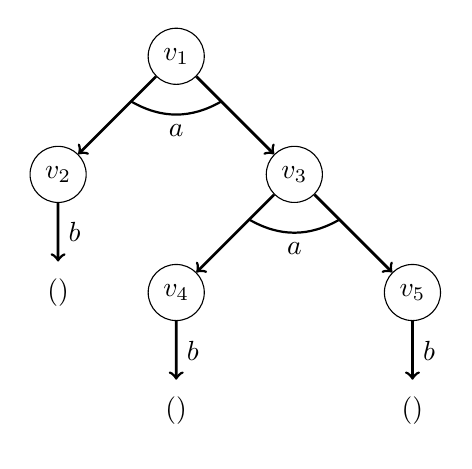
\begin{tikzpicture}[
  scale=0.8,
  node distance = 1.5cm,
  tnode/.style={circle, text centered, draw=black},
  lnode/.style={circle, text centered},
  arw/.style={->, line width=1pt},
  symline/.style={-, line width=0.8pt}
  ]

\node [tnode] (v1) {$v_1$};
\node [tnode, left of=v1, below of=v1] (v2) {$v_2$};
\node [left of=v1, below of=v1, above of=v2, right of=v2, yshift=1cm, xshift=0.8cm] (v1v2) {};
\node [tnode, right of=v1, below of=v1] (v3) {$v_3$};
\node [left of=v1, below of=v1, above of=v3, right of=v3, yshift=1cm, xshift=-0.8cm] (v1v3) {};
\node [lnode, below of=v2] (v02) {$()$};

\node [tnode, below of=v3, left of=v3] (v4) {$v_4$};
\node [left of=v3, below of=v3, above of=v4, right of=v4, yshift=1cm, xshift=0.8cm] (v3v4) {};
\node [tnode, below of=v3, right of=v3] (v5) {$v_5$};
\node [left of=v3, below of=v3, above of=v5, right of=v5, yshift=1cm, xshift=-0.8cm] (v3v5) {};
\node [lnode, below of=v4] (v04) {$()$};
\node [lnode, below of=v5] (v05) {$()$};

\draw [arw] (v1) -- (v2);
\draw [arw] (v1) -- (v3);
\draw [arw] (v2) -- node [midway, right] {$b$} (v02);
\draw [arw] (v3) -- (v4);
\draw [arw] (v3) -- (v5);
\draw [arw] (v4) -- node [midway, right] {$b$} (v04);
\draw [arw] (v5) -- node [midway, right] {$b$} (v05);

\draw [symline] (v1v2) edge [bend right] node [midway, below] {$a$} (v1v3);
\draw [symline] (v3v4) edge [bend right] node [midway, below] {$a$} (v3v5);

\end{tikzpicture}

		\end{center}
		\caption{A graph $t$ that has attributes of a tree.}
		\label{fig:graph_tree}
	\end{figure}
	\label{ex:graph}
\eexmp

\subsection{Forests}
\label{subsec:forests}

Let us suppose without loss of generality that $\Sigma \cap \mathbb{N} = \emptyset$.
A $\Sigma$-labelled \emph{forest} is a sequence of trees $t_1 \cdots t_n$ over ($\Sigma \cup \{1,\ldots,n\}$)
where $\forall i \in \{1,\ldots,n\}: \#i = 0$.
\emph{Root references} are leaves labelled by $i \in \mathbb{N}$.
The forest $t_1 \cdots t_n$ (we suppose that the sets of nodes of the trees are disjoint) represents the graph $\fagr$ that could
be constructed by interconnecting roots by the related root reference.
E.g., a root reference $2$ in $t_1$ would be replaced by the root node of $t_2$.
Let's formalize the idea of construction of $\fagr$.
$\fagr$ contains an edge $v \mapsto (a,v_1 \cdots v_m)$ iff $\exists i \in \{1, \ldots, n\} \ \exists(v \mapsto (a, v_1' \cdots v_m')) \in edges(t_i)
\ \forall j \in \{1,\ldots,m\}: v_j = h(v_j')$ where $edges(t_i)$ is the set of all edges of the tree $t_i$ and
\[ h(v_j') = \left\{
  \begin{array}{l l}
  root(t_k) & \quad \text{if $v_j'$ is a root reference with $l(v_j') = k$}\\
  v_j'   & \quad \text{otherwise}
  \end{array} \right.\]

\pagebreak
\bexmp
We illustrate the notion of forest in an example.
Consider a forest $f$ in Figure \ref{fig:forest}.
The forest $f$ consists three trees, $t_1$ with a root $u_1$,
$t_2$ with a root $v_1$ and $t_3$ with a root $w_1$.
The alphabet $\Sigma$ of the trees is same as in Example \ref{ex:graph} but $f$
is defined over $\Sigma \cup \{\overline{2}, \overline{3}\}$
where $\overline{2}, \overline{3}$ denotes the root references $u_5$, $v_3$.
to the second and the third tree.

We can obtain a graph $\otimes t_1,t_2,t_3$ shown in Figure from $t_1, t_2, t_3$.
The edges with root references are replaced by another edges leading to the roots
of the referenced trees.
A created graph is in Figure \ref{fig:forest_graph}.

	\begin{figure}[bth]
	\begin{center}
		\scalebox{1}
		{
			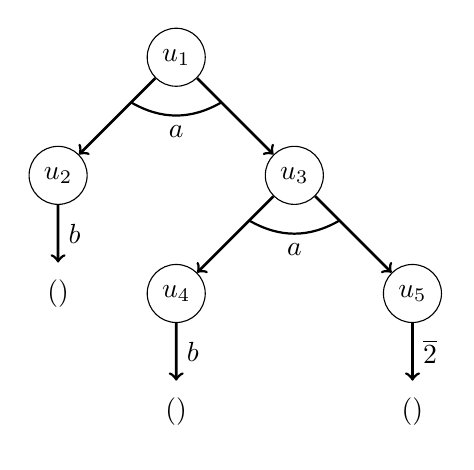
\begin{tikzpicture}[
  scale=0.8,
  node distance = 1.5cm,
  tnode/.style={circle, text centered, draw=black},
  lnode/.style={circle, text centered},
  arw/.style={->, line width=1pt},
  symline/.style={-, line width=0.8pt}
  ]

\node [tnode] (u1) {$u_1$};
\node [tnode, left of=u1, below of=u1] (u2) {$u_2$};
\node [left of=u1, below of=u1, above of=u2, right of=u2, yshift=1cm, xshift=0.8cm] (u1u2) {};
\node [tnode, right of=u1, below of=u1] (u3) {$u_3$};
\node [left of=u1, below of=u1, above of=u3, right of=u3, yshift=1cm, xshift=-0.8cm] (u1u3) {};
\node [lnode, below of=u2] (u02) {$()$};

\node [tnode, below of=u3, left of=u3] (u4) {$u_4$};
\node [left of=u3, below of=u3, above of=u4, right of=u4, yshift=1cm, xshift=0.8cm] (u3u4) {};
\node [tnode, below of=u3, right of=u3] (u5) {$u_5$};
\node [left of=u3, below of=u3, above of=u5, right of=u5, yshift=1cm, xshift=-0.8cm] (u3u5) {};
\node [lnode, below of=u4] (u04) {$()$};
\node [lnode, below of=u5] (u05) {$()$};

\draw [arw] (u1) -- (u2);
\draw [arw] (u1) -- (u3);
\draw [arw] (u2) -- node [midway, right] {$b$} (u02);
\draw [arw] (u3) -- (u4);
\draw [arw] (u3) -- (u5);
\draw [arw] (u4) -- node [midway, right] {$b$} (u04);
\draw [arw] (u5) -- node [midway, right] {$\overline{2}$} (u05);

\draw [symline] (u1u2) edge [bend right] node [midway, below] {$a$} (u1u3);
\draw [symline] (u3u4) edge [bend right] node [midway, below] {$a$} (u3u5);

\end{tikzpicture}

			\hspace{0.55cm}
			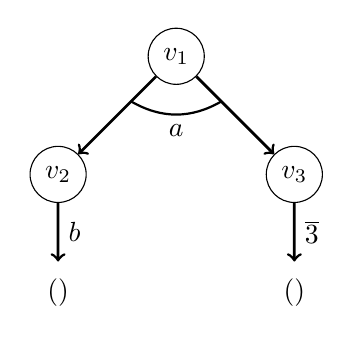
\begin{tikzpicture}[
  scale=0.8,
  node distance = 1.5cm,
  tnode/.style={circle, text centered, draw=black},
  lnode/.style={circle, text centered},
  arw/.style={->, line width=1pt},
  symline/.style={-, line width=0.8pt}
  ]

\node [tnode] (v1) {$v_1$};
\node [tnode, left of=v1, below of=v1] (v2) {$v_2$};
\node [left of=v1, below of=v1, above of=v2, right of=v2, yshift=1cm, xshift=0.8cm] (v1v2) {};
\node [tnode, right of=v1, below of=v1] (v3) {$v_3$};
\node [left of=v1, below of=v1, above of=v3, right of=v3, yshift=1cm, xshift=-0.8cm] (v1v3) {};
\node [lnode, below of=v2] (v02) {$()$};
\node [lnode, below of=v3] (v03) {$()$};

\draw [arw] (v1) -- (v2);
\draw [arw] (v1) -- (v3);
\draw [arw] (v2) -- node [midway, right] {$b$} (v02);
\draw [arw] (v3) -- node [midway, right] {$\overline{3}$} (v03);

\draw [symline] (v1v2) edge [bend right] node [midway, below] {$a$} (v1v3);

\end{tikzpicture}

			\hspace{0.55cm}
			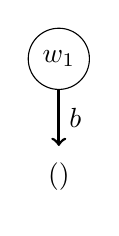
\begin{tikzpicture}[
  scale=0.8,
  node distance = 1.5cm,
  tnode/.style={circle, text centered, draw=black},
  lnode/.style={circle, text centered},
  arw/.style={->, line width=1pt},
  symline/.style={-, line width=0.8pt}
  ]

\node [tnode] (w1) {$w_1$};
\node [lnode, below of=w1] (w01) {$()$};

\draw [arw] (w1) -- node [midway, right] {$b$} (w01);

\end{tikzpicture}

		}
		\caption{A forest $f$ constisting the three trees $t_1, t_2, t_3$ with roots $u_1, v_1, w_1$}.
	  \label{fig:forest}
	\end{center}
	\end{figure}

	\begin{figure}[bth]
	\begin{center}
		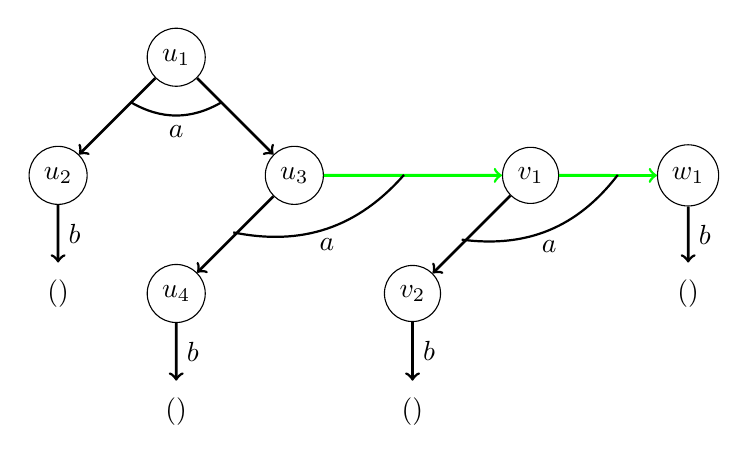
\begin{tikzpicture}[
  scale=0.8,
  node distance = 1.5cm,
  tnode/.style={circle, text centered, draw=black},
  lnode/.style={circle, text centered},
  arw/.style={->, line width=1pt},
  symline/.style={-, line width=0.8pt}
  ]

% tree 1

\node [tnode] (u1) {$u_1$};
\node [tnode, left of=u1, below of=u1] (u2) {$u_2$};
\node [left of=u1, below of=u1, above of=u2, right of=u2, yshift=1cm, xshift=0.8cm] (u1u2) {};
\node [tnode, right of=u1, below of=u1] (u3) {$u_3$};
\node [left of=u1, below of=u1, above of=u3, right of=u3, yshift=1cm, xshift=-0.8cm] (u1u3) {};
\node [lnode, below of=u2] (u02) {$()$};

\node [tnode, below of=u3, left of=u3] (u4) {$u_4$};
\node [left of=u3, below of=u3, above of=u4, right of=u4, yshift=0.8cm, xshift=0.6cm] (u3u4) {};
\node [lnode, below of=u4] (u04) {$()$};

\node [right of=u3, left of=v1, right of=u1, below of=u1, xshift=1.5cm, yshift=0.13cm] (u3v1) {};

\draw [arw] (u1) -- (u2);
\draw [arw] (u1) -- (u3);
\draw [arw] (u2) -- node [midway, right] {$b$} (u02);
\draw [arw] (u3) -- (u4);
\draw [arw] (u4) -- node [midway, right] {$b$} (u04);

\draw [symline] (u1u2) edge [bend right] node [midway, below] {$a$} (u1u3);

% tree 2
\node [tnode, right of=u1, right of=u3] (v1) {$v_1$};
\node [tnode, left of=v1, below of=v1] (v2) {$v_2$};
\node [left of=v1, below of=v1, above of=v2, right of=v2, yshift=0.7cm, xshift=0.5cm] (v1v2) {};
\node [lnode, below of=v2] (v02) {$()$};

\draw [arw] (v1) -- (v2);
\draw [arw] (v2) -- node [midway, right] {$b$} (v02);

%tree 3
\node [tnode, right of=v1, xshift=0.5cm] (w1) {$w_1$};
\node [lnode, below of=w1] (w01) {$()$};
\node [right of=v1, left of=w1, yshift=0.13cm, xshift=-0.8cm] (v1v3) {};

\draw [arw] (w1) -- node [midway, right] {$b$} (w01);

%\draw [arw] (w1) -- node [midway, right] {$b$} (w01);

%connection

\draw [arw, color=green] (u3) -- (v1);
\draw [arw, color=green] (v1) -- (w1);

\draw [symline] (u3u4) edge [bend right] node [midway, below] {$a$} (u3v1);
\draw [symline] (v1v2) edge [bend right] node [midway, below] {$a$} (v1v3);

\end{tikzpicture}

		\caption{A graph $\otimes t_1,t_2,t_3$ obtained from a forest in Figure \ref{fig:forest}.
		The green edges are the ones added to create the graph from forest}.
	  \label{fig:forest_graph}
	\end{center}
	\end{figure}
\eexmp

\subsection{Graphs and Forests with Ports}
\label{subsec:gfp}

We extend graphs and forests with concept of \emph{ports} which should
serve for marking input and output nodes.
An \emph{input-output-graph} (io-graph) is a pair $(g,\phi)$ (in sense of brevity also denoted by $g_\phi$)
where $g$ is a graph and $\phi=(\phi_1 \cdots \phi_n) \in dom(g)^+$ is a sequence of ports, $\phi_1$
is an input port and $\phi_1 \cdots \phi_n$ is a sequence of output ports.
The ports in $\phi$ are unique.
If a root of $g_\phi$ is $\phi_1$ then $g_\phi$ is called \emph{accessible}.

The \emph{cut-points} of a graph $g_\phi$ is the set of its ports and joins and we denote this set by $cps(g_\phi)$.
Formally, $cps(g_\phi)=\{v \in V\,|\, v \in \phi \vee idg(v) > 1\}$.

An \emph{io-forest} is a pair $f=(t_1 \cdots t_n, \pi)$ such that $n \geq 1$ and $\pi \in \{1,\ldots,n\}^n$
is a sequence of port indices, where $\pi_1$ is a input port index and $\pi_2 \ldots \pi_{|\pi|}$ is a sequence
of the output ports indices.
As in the case of the ports the indices are unique.
It is also possible to construct an io-graph $\otimes f$ from a forest $f$ such that
$\otimes f = (\otimes t_1 \cdots t_n,root(t_{\pi_{1}},\ldots,t_{\pi_{n}}))$.
So the ports of $\otimes f$ are roots of the trees indexed by indices in $\pi$.
This means that a root of the tree pointed by $\pi_1$ is an input port of $\otimes f$ and
the roots of the trees pointed by the other indices in $\pi$ are the output ports of $\otimes f$.

\bexmp
Recall graph $t$ from Figure \ref{fig:graph_tree}.
We can extend it to a io-graph $t_\phi$ where $t$ is unchanged and
$\phi=(v_1,v_4,v_5)$ (of course, there are different ways how to define the ports).
The io-graph $t_\phi$ has an input port $v_1$ and the output ports are $v_2,v_3$.
Because $v_1$ is the root the tree $t_\phi$ is accesible.
The cutpoints of $t_\phi$ are $v_1, v_4, v_5$.

In Figure \ref{fig:forest} we shown the forest $f$.
This forest could be extended to a io-forest $f_{io}=((t_1,t_2,t_3),\pi)$ by defining sequence of port indices $\pi$
which could be e.g., $(1,3)$.
Then a graph $\otimes f_{io}$ is a pair $(\otimes (t_1,t_2,t_3)$, $(u_1,w_1))$.
The graph $\otimes (t_1,t_2,t_3)$ is the same as in Figure \ref{fig:forest_graph}.
The inpurt port $u_1$ is related to the input port index $1$ of $f_{io}$
and the output port $w_1$ is related to the output port index $3$.
\label{ex:iograph}
\eexmp

\subsection{Minimal and Canonical Forest}
\label{subsec:mcforest}

There are two properties of the forests, minimality and canonicity, that we will further employ.
The properties make possible to represent an io-forest in unique way.
That enables manipulating with io-forest it in deterministic way.
An io-forest $f_m=(t_1 \cdots t_n, \phi)$ representing a graph $\otimes f$ is \emph{minimal}
iff the roots of trees $t_1,\ldots,t_n$ corresponds to the cut-points of $\otimes f$,
so there is a bijection between $\{root(t_k)\,|\, t_k \in \{t_1, \ldots, t_n\} )\}$ and $cps(\otimes f)$.
The minimal io-forest is unique up-to to permutations of $t_1,\ldots,t_n$.

We need to defined ordering $\preceq_p$, so called \emph{canonical ordering}, over cut-points of $\otimes f$ to be able to define canonicity of the forest $f$.
The canonical ordering $\preceq_p \subseteq cps(\otimes f) \times cps(\otimes f)$ is defined as follows: $c_1 \preceq_p c_2 \Leftrightarrow \emph{the cost of the cheapest path from }
\phi_1 \emph{ (input port) to } c_1 \emph{ is}$ $\emph{cheaper}$ $\emph{ than the cost of the cheapest path from } \phi_1 \emph{ to } c_2$.
The io-forest $f_c$ is \emph{canonical} iff it is minimal, the trees $t_1,\ldots, t_n$ are ordered by $\preceq_p$, and $\otimes f$ is accessible.
The canonical io-forest is a unique representation of a accessible io-graph.
The canonical io-forest can be obtained by depth-first traversal (DFT)\cite{taocp} of $\otimes f$.
We need to assume that there is an ordering $\leq_\Sigma$ over labels $\Sigma$ of $\otimes f$ before description of DFT method to
make DFT traversal deterministic and hence the ordering of the trees unique.
We create a stack of nodes initialized with input and output ports ordered by $\preceq_p$ when the smallest node is on the top of the stack.
Then the DFT is run over $\otimes f$ and we obtain canonical forest $f_c$ where trees are in the following order.
The first ones are trees corresponding to the ports of $f$ ordered by $\preceq_p$ and the rest of the trees are in the order
in which they were visited by DFT traversal.


\subsection{Tree Automata}
\label{subsec:ta}

A (finite, non-deterministic, top-down) \emph{tree automaton} (TA) is a
quadruple $A = (Q, \Sigma, \Delta, R)$ where
\begin{itemize}
	\item $Q$ is a finite set of \emph{states}
	\item $\Sigma$ is a ranked alphabet
	\item $\Delta$ is a set of \emph{transition rules} where transitions have a form $(q,a,q_1 \cdots q_n)$ where $q,q_1,\ldots,q_n \in Q$, $a \in \Sigma$, $n \geq 0$ and $\#a = n$.
		Alternatively, we write $q \xrightarrow{a} (q_1 \cdots q_n)$ to denote a $(q,a,q_1 \cdots q_n) \in \Delta$.
		When $n=0$ then the rule is called \emph{leaf rule}.
	\item $R \subseteq Q$ is a set of \emph{root states}.
\end{itemize}

We could symmetrically define also bottom-up tree automata as quadruple $B = (Q, \Sigma, \Delta, F)$ where
\begin{itemize}
	\item $Q$ is a finite set of states
	\item $\Sigma$ is a ranked alphabet
	\item $\Delta$ is a set of transition rules where transition has a form $(q_1 \cdots q_n,a,q)$ where $q,q_1,\ldots,q_n \in Q$, $a \in \Sigma$, $n \geq 0$ and $\#a = n$.
		We can again write $(q_1 \cdots q_n) \xrightarrow{a} q$ to denote a $(q_1 \cdots q_n,a,q) \in \Delta$.
		When $n=0$ then the rule is called \emph{leaf rule}.
	\item $F \subseteq Q$ is a set of \emph{final states}.
\end{itemize}

We will further consider top-down tree automata as default.

Now the semantics of TA will be defined.
A \emph{run} of $A$ over a tree $t$ is mapping $\funcdecl{\rho}{dom(t)}{Q}$ such that
$\forall v \in dom(t)\ \exists (q \xrightarrow{a} (q_1 \cdots q_n)) \in \Delta:  q=\rho(v) \wedge  \forall i \in \{1, \ldots, |S(v)|\}: q_i=\rho(S(v)_i)$.
We use $t \Rightarrow_{\rho} q$ to denote a run $\rho$ of $A$ over tree $t$ s.t. $\rho(root(t)) = q$ and we use $t \Rightarrow q$ to denote that there exists
run $\rho$ over $t$ to $q$.
Finally, we can define the language of $A$.
The \emph{language} of a state $q\in Q$ is defined by $L(q) = \{t\,|\, t \Rightarrow q\}$.
The \emph{language} of $A$ is defined by $L(A) = \bigcup_{q\in R} L(q)$.

\bexmp
Let define a tree automata $A=(Q,\Sigma,\Delta, R)$
where $Q=\{q_1,q_2,q_3,q_4,q_5\}$, $\Sigma = \{a,b\}$,
such that $\#(a) = 2, \#(b) =0$, $R=\{q_1\}$,
and $\Delta=\{q_1 \xrightarrow{a} (q_2,q_3), q_2 \xrightarrow{b} (),
q_3 \xrightarrow{b} (q_4,q_5), q_4 \xrightarrow{b} (), q_4 \xrightarrow{b} ()\}$.
Then a run $\rho$ of $A$ over the tree $t$ from Figure \ref{fig:graph_tree}
is defined as follows: $\forall i \in \{1,\ldots,5\}: \rho(v_i) = q_i$.
Since $\rho(root(t)) = \rho(v_1) = q_1$ then $t \in L(q_1)$ and becasue $q \in R$
it also holds $t \in L(A)$.
\label{ex:ta}
\eexmp

\subsection{Forest Automata}
\label{subsec:fa}

A \emph{Forest Automata} (FA) over $\Sigma$ is a pair $F=(A_1\cdots A_n, \pi)$
where $A_1 \cdots A_n$ is a sequence of tree automata defined over the alphabet $\Sigma \cup \{1,\ldots,n\}$
and $\pi = I_1 \cdots I_n$ where $I_1,\ldots, I_n \in \{1, \ldots, n\}$ is a sequence of port indices.
There are two kinds of languages related to FA.
The first one is forest language obtained by Cartesian product of the languages of particular TA (and port indices) of FA
and hence the forest language is a set of the io-forests.
The second one is the graph language obtained by connecting the io-forests from forest language to io-graphs.
Formally, the \emph{forest language} of the FA $F$ is the set of io-forests $L_f(F)= L(A_1) \times \ldots L(A_n) \times \{\pi\}$.
Note that it is necessary to add to the Cartesian product also the sequence of indices to preserve structure of io-forests
and hence to be able to construct graph language of $F$ in deterministic way.
The \emph{graph language} of $F$ is the set of io-graph $L(F) = \{\otimes f\,|\, f \in L_f(F)\}$.
We say that $F$ respects \emph{canonicity} if $\forall f \in L_f(F): \emph{f is canonical}$.

One of the most important operation over forest automata performed in analysis of a program is checking
language inclusion of two forest automata.
This operation is performed to check whether a fixpoint in a program point is reached during symbolic execution.
Checking inclusion of languages of forest automata respecting canonicity could be done \emph{component-wise},
i.e. checking language inclusion of their tree automata one by one.

\begin{lemma}
	Let $F^1 = (A_1^1\cdots A_{n_{1}}^1, \pi^1)$ and $F^2 = (A_1^2\cdots A_{n_{2}}^2, \pi^2)$
	be two FA respecting canonicity.
	Then $L(F^1) \subseteq L(F^2)$ iff
	\begin{itemize}
			\item $n_1$ = $n_2$
			\item $\pi^1 = \pi^2$
			\item $\forall i \in \{1,\ldots,n_1\}: L(A_i^1) \subseteq L(A_i^2)$
	\end{itemize}
\end{lemma}
\begin{proof}
	Proof can be found in \cite{forester:techrep}.
\end{proof}

\bexmp
We consider the io-forest $f_{io}=((t_1,t_2,t_3), (1,3))$ from Example \ref{ex:iograph}.
The tree $t_1$ (which is the same as the tree $t$) belongs to the language of TA $A$
defined in Example \ref{ex:ta}.
We further define a TA $B=(Q_B,\Sigma, \Delta_B, R_B)$ where $Q_B=\{p_1,p_2,p_3\}$,
$\Sigma$ is same as in Example \ref{ex:ta},
$\Delta=\{p_1 \xrightarrow{a} (p_2,p_3),
p_2 \xrightarrow{b} (),
p_3 \xrightarrow{b} ()\}$
and $R\{p_1\}$.
TA $B$ has $t_2$ in its language.
Finally, we define a TA $C=(Q_C,\Sigma, \Delta_C, R_C)$ where $Q_C=\{r_1\}$,
$\Sigma$ is again the same as before,
$\Delta= r_1 \xrightarrow{b} ()\}$
and $R\{r_1\}$.
A set $L(C)$ contains $t_3$.
Putting all defined automata together we can construct a forest automata $F=((A,B,C),(1,3))$.
The io-forest $f_{io}$ is in the forest language $L_f(F)$ of $F$ because it belongs
to $L(A) \times L(B) \times L(C) \times \{(1,3)\}$.
Hence the graph $\otimes f_{io} = (\otimes (t_1,t_2,t_3),(u_1,w_1))$
(also defined in Example \ref{ex:iograph}) is in the graph language $L(F)$.
\eexmp

\section{Forest Automata of Higher Level}
\label{sec:fah}

We are able to represent some data structures, like singly-linked lists or trees, by already defined forest automata
but we need to define hierarchical forest automata to be able to represent
another class of data structures (further described in \ref{subsec:boxes}), like doubly-linked lists or trees with root pointers.
For creating the hierarchy of forest automata we need to introduce \emph{structured labels}.
This labels could contain another forest automata.
The hierarchy then comes from the fact that forest automata of a certain level
are defined over structured labels containing FA of lower levels.

\subsection{Structured Labels}

$\Gamma$ is a ranked alphabet of \emph{sub-labels} with defined total ordering $\sqsubset$.
Let $g$ be a graph defined over $2^\Gamma$ where $A$ denotes a symbol of $g$ and $\forall A \subseteq \Gamma: \#A = \sum_{a\in A} \#a$.
The graph $g$ has edges in the form $v \mapsto (\{a_1,\ldots,a_m\},v_1 \cdots v_n)$ where
$a_1 \sqsubset a_2 \sqsubset \ldots \sqsubset a_m$ and $\sum_{a \in \{a_1,\ldots,a_n\}} \# a = n$.
We denote such edge by $e$.
Each edge $e$ consists \emph{sub-edges} that creates sequence $e\langle 1\rangle = v \mapsto (a_1,v_1 \cdots v_{\#a_1}) \cdots e\langle n\rangle= v \mapsto (a_m,v_{n-\#a_m+1} \cdots v_m)$.
We denote $i$-th sub-edge of $e$ in $g$ by $e\langle i\rangle = v \mapsto (a_i,v_k \cdots v_l)$ where $i \in \{1,\ldots,m\}$ or
we can also denote it by indices from $\{k,\ldots,l\}$.
We use $SE(g)$ to denote all sub-edges of graph $g$.
A node $v$ of a graph is \emph{isolated} if it is not part of any sub-edge.
Formally, a node $v$ is isolated iff $\nexists\, e\langle i\rangle = v' \mapsto (a_i,v_k \cdots v_l): v = v' \wedge \nexists\, e\langle i\rangle = v' \mapsto (a_i,v_k \cdots v_l)\ \exists v'' \in \{v_k,\ldots, v_l\}: v = v''$.
A graph $g$ is \emph{unambiguously determined} by $SE(g)$ if $g$ has no isolated nodes.

\subsection{Tree Automata over Structured Labels}

Since we already extended the labels to structures ones we also define tree automata over these labels.
A (finite, non-deterministic, top-down) \emph{tree automata} (over structured labels) is quadruple $A=(Q,2^\Gamma, \delta, R)$ where
\begin{itemize}
	\item $Q$ is a finite set of states.
	\item $\Gamma$ is a ranked alphabet.
	\item $\Delta$ is a set of transition rules set with rules in the form $(q,\{a_1,\ldots,a_m\},q_1 \cdots q_n)$ where $q,q_1,\ldots,q_n \in Q$, $\{a_1,\ldots,a_m\} \in \Gamma$.
	Each rule could be interpreted as a sequence of the \emph{rule-terms} $d\langle 1\rangle = q \mapsto (a_1,q_1 \cdots q_{\#a_1}) \cdots d\langle n\rangle= q \mapsto (a_m,q_{n-\#a_m+1} \cdots q_n)$ and
	we denote the $i$-th rule term of sequence again by $d\langle i\rangle$ where $i \in \{1,\ldots,m\}$.
	\item $R\subseteq Q$ is a finite set of root states.
\end{itemize}

\subsection{Forest Automata of Higher Level}

Finally, we can extend also FA to a version defined over structured labels.
Informally, a forest automaton of a higher level has another forest automata (of lower lever) as the symbols on its edges.
This makes possible to build a hierarchy of forest automata.
Let formalize this idea.
We start from forest automata of \emph{level} 1.
So let $\Gamma_1$ be a set of all forest automata over $2^\Gamma$ and let the elements of this set be called \emph{forest automata of level 1}.
All forest automata of \emph{level $i$} form the set $\Gamma_i$.
A forest automaton $F$ of level $i$ is defined over the ranked alphabet $2^{\Gamma \cup \Delta}$ where $\Delta$ is a subset of forest automata of
level $i-1$ which are called \emph{boxes} of $F$.
The \emph{Rank} $F$ of an FA $F$ is the number of its output port indices.
Finally, the set of all forest automata of all levels $\sum_{i \geq 0} \Gamma_i$ is denoted by $\Gamma^{*}$ and it is ordered by a total ordering $\sqsubset_{\Gamma_*}$.

We define operation \emph{sub-edge replacement} which help us to define semantics of forest automata of higher level.
Informally, the sub-edge replacement removes a sub-edge and matches its origin and outputs with a new graph serving like a substitution of the sub-edge.
This operation will be further used for replacement of sub-edge of FA with by a graph represented by FA of lower level.

Formally, let $g$ be a graph with an edge $e \in edges(g)$ and sub-edge $e\langle i\rangle = v_1 \rightarrow (a,v_2 \cdots v_n)$.
Let $g_{\phi}'$ be an io-graph such that $|\phi| = n$.
We assume that $dom(g) \cap dom(g') = \emptyset$.
The sub-edge $e\langle i\rangle$ could be replaced by $g'$ such that $\forall j \in \{1,\ldots,n\}: l_{g}(v_j) \cap
l_{g'}(\phi_j) = \emptyset$
(this conditions checks whether there is no successor of $v_j$ and $\phi_j$ reachable over the same
label from both nodes).
The result of replacement (if it is possible to do it) is denoted as $g\subst{g'_\phi}{e\langle i\rangle}$.
The result is the graph $g_n$ in a sequence $g_0 \cdots g_n$ of graphs which are defined as follows: 
\begin{itemize}
	\item $SE(g_0) = SE(g) \cup SE(g') \setminus \{e\langle i\rangle\}$.
	\item $\forall j \in \{1, \ldots, n\}: \emph{the graph } g_j \emph{ is obtained from } g_{j-1} \emph{ by following procedure }$
		\begin{enumerate}
			\item Deriving a~graph $h$ by replacing the origin of the sub-edges of the $j$-th port $\phi_j$ of $g'$ by $v_j$.
			\item Redirecting edges leading to $\phi_{j}$ to $v_j$, i.e., replacing all occurrences of $\phi_j$ in $rng(h)$ by $v_j$
			\item Removing $\phi_j$. 
		\end{enumerate}
\end{itemize}

We apply the concept of sub-edge replacement to the forest automata of higher level now
and introduce following two procedures over FA.
\begin{itemize}
	\item \emph{Unfolding} of a graph $g$ is replacement of its sub-edge with a symbol, which is
		a FA $F'$, by a graph from $L(F')$.
		Formally, sub-edge $e\langle i \rangle$ of the graph $g$ has a symbol $a$ and this symbol is a FA $F'$ (so this symbol is a box)
		and $g'_\phi \in L(a)$ then $h = g \subst{g'_\phi}{e\langle i \rangle}$ is an unfolding of $g$.
		We denote unfolding $h$ of $g$ by $g \prec h$.
	\item \emph{Folding} is a replacement of $g'_\phi$ by $e \langle i \rangle$ in $h$ obtaining $g$.
		So we can say that $g'_\phi$ is folded to $e \langle i \rangle$. 
\end{itemize}

A transitive reflective closure of $\prec$ is denoted by $\prec^*$.
A set of all graphs obtained by repeated application of unfolding from
a graph $g$ over ranked alphabet $\Gamma$ is called \emph{$\Gamma$-semantics}. 
\emph{$\Gamma$-semantics} is formally defined as a set of graphs $g'$ such that $g \prec^* g'$.
We denote it as $\llbracket g \rrbracket_\Gamma$ or just simply $\llbracket g \rrbracket$ when it is
clear which alphabet we speak about.
Finally, \emph{$\Gamma$-semantics} is defined for a FA $F$ of higher level as follows $\llbracket F \rrbracket = \bigcup_{g_\phi \in L(F)} (\llbracket g \rrbracket \times \{\phi\})$.
Please note that the the meaning of $L(F)$ and $L_f(F)$ has not been changed so the both sets (languages) can contain just graphs (or forests)
over structured labels.

When we recall the definition of canonicity respecting FA we will find that it is applicable also for FA of higher level.
A FA $F$ is canonicity respecting if $\forall f \in L_f(F): \emph{f is canonical}$ and since definition of canonical $f$
is not affected by extending labels to the structured ones the meaning of canonicity is same as for basic FA.
The language inclusion checking is again possible in component-wise way like in the case of basic FA what is
proofed in \cite{forester:techrep}.

%TODO sets of FA. are they really needed anywhere?

\chapter{Forest Automata based Verification}
\label{ch:fav}

The different heap configurations could be reached during execution of a program.
The aim of the shape analysis is to prove that it is not possible to reach such a heap configuration in which
an error like double free or invalid pointer can occur.
The heap configurations could be represented by FA and hence it is possible
to use FA in shape analysis.

This chapter provides an overview of the shape analysis based forest automata introduced in \cite{forester12}.
First, a heap representation using FA is described and then
we provide overview of symbolic execution that employs framework of abstract interpretation.

\section{Heap Representation}
\label{sec:hd}

It is possible to view a \emph{heap} (more precisely, a single heap configuration)
as a (directed) graph where each allocated heap cells corresponds to a node in the graph \cite{forester13}.
The heap cells consists of \emph{pointer selectors} and \emph{data selectors} that picks a data from some finite data domain.
A pointer selectors could point to another graph node or to the value \emph{null} or it could be undefined.
A data selector then references its node to the data from data domain.
%When we consider the pointer variables of a program it also holds that they can have pointer and data selectors.
A heap graph could be split to the trees in the following manner.
We identify the heap cut-points (corresponding to the already defined term \emph{cut-points})
which are the heap cells pointed by a pointer variable or by more then one other heap cells by their pointer selectors.
The heap is then split to the trees whose roots nodes are cut-points identified in the previous step.
The pointer selectors that pointed to the cut-points are redirected to the corresponding root references which interconnects
particular tree components (and provides possibility to reconstruct the original graph again).
Finally, the created tuple of the trees is called a forest.
Please note, that the mentioned procedure corresponds to the terms defined in Chapter \ref{ch:prel}
so it is possible to achieve canonical forest as it was described in Section \ref{subsec:mcforest}.

Let us formalize the idea given above.
We denote a pointer selector by $PSel$, a data selector by $DSel$ and data domain by $\mathbb{D}$ \cite{techrep}.
A single heap configuration is a io-graph $g_{st}$ over the ranked alphabet of the structured labels from $2^\Gamma$
with sub-labels from the ranked alphabet $\Gamma = PSel \cup (DSel \times \mathbb{D})$ having the
ranking function that assigns $1$ to the pointer selectors and $0$ to the data selectors.
The values of data selectors are stored in the structured labels as sub-labels from $DSel \times \mathbb{D}$.
A node $v$ of a graph representing a heap reflects by its label internal structure the structure of
related allocated memory cell in the heap so it holds that $l_g(v) \in 2^\Gamma$.
A null value is represented by a node $\texttt{null}$ with $l_g(\texttt{null}) = \emptyset$
and undefined selectors of a node $v$ have not corresponding  sub-labels in $l_g(\texttt{v})$.

\bexmp
We illustrate described principle of heap representation with an example taken from \cite{techrep}.
We consider a singly-linked list whose items are data structures containing pointers to
a next item and also integer data variable, written in C:
\begin{center}
\begin{minipage}{0.3\textwidth}
    \begin{verbatim}
     struct SLL {
      struct SLL* next;
      int data;
     };
    \end{verbatim}
\end{minipage}
\end{center}
Then a allocated cell of this singly-linked list on the heap with value $13$ in \texttt{data} variable and pointer to a cell named $s_{next}$
in \texttt{next} variable could be represented
by a node $s$ with following label $l_g(s) = \{next_g(s_{next}),(data_g,13),()\}$.
As you can see, the pointer selector $next_g \in PSel$ representing the pointer variable \texttt{next} from \texttt{SLL} structure
has really rank $1$ and sub-label $(data_g,13) \in DSel\times \mathbb{D}$ representing \texttt{data} variable from \texttt{SLL} structure
has rank $0$.
\eexmp

We need to represent the sets of the heap configurations reachable by the analysed program, not only single heap configuration.
That would be possible by employing the forest automata of higher level respecting canonicity that represents io-forests
which model the set of heap configurations.

The another thing needed to be represented by FA is a \emph{stack frame} of a function in the analyzed program.
When we recall definition of io-forests and forest automata so they contains exactly one (index of) input port.
The input port node $sf$ serves in case of shape analysis based on FA for storing of a stack frame of the analyzed function.

\section{Symbolic Execution}
\label{sec:se}

FA-based verification procedure is a standard \emph{abstract interpretation} \cite{cousot:77}.
The concrete domain assigns to each program location a set of pairs
$(\sigma,H)$ where a mapping $\sigma$ maps each variable
to a node in $H$, to a $\texttt{null}$ or to an undefined value, and $H$ is a single heap configuration.
The abstract domain than assigns to each program location a finite set of pairs
$(\sigma, F)$ (called \emph{abstract configuration}) where $\sigma$ maps again each variable to a
$\texttt{null}$ value or to undefined value or to an index of TA in $F$ and $F$ is a forest automata
of higher level respecting canonicity representing a set of heaps configurations.
Note that a set of FA is needed in abstract domain to represent one program locations (since
abstract domain maps to the set of abstract configurations).
FA are not closed under union so it is not possible to represent the sets of heaps by single FA.

The verification starts from initial abstract configuration that consists an FA for initial heap configuration representing io-graph
$g_{\mathit{sf}}$ where $g$ consists from two nodes.
The first one is $\texttt{null}$ and the second one is empty stack frame $sf$ with $l_g(\mathit{sf}) = \emptyset$.
The sequence of \emph{abstract transformers} related to the program statements is then iteratively applied to the abstract configurations.
The process of applying abstract transformers over abstract domain is called \emph{symbolic execution}.
As it was said, each abstract transformer correspond to a statement of the analyzed program.
It is possible to define a function $f_{\texttt{op}}(g_{st})$ related to an operation \texttt{op} from the intermediate code of the analysed program.
This function models semantics of \texttt{op} in concrete domain in such way that $f_{\texttt{op}}(g_{\mathit{st}})$
returns an io-graph representing the heap configuration obtained after execution of the concrete operation \texttt{op} over concrete domain.
The abstract transformers $\tau_{\texttt{op}}$ are defined for each concrete operation \texttt{op} reflecting semantics of $f(\texttt{op})$.
The abstract transformer $\tau_{\texttt{op}}$ applied to a FA $S$ representing heap in abstract domain returns a result FA $S' = \tau_{\texttt{op}}(S)$
such that $\bigcup_{F' \in S'} \llbracket F' \rrbracket = \{ f_{\texttt{op}}(g_{sf}) \,|\, g_{sf} \in \llbracket F \rrbracket \wedge F \in S \}$.
The abstract transformer is applied separately to each forest $F \in S$.

The abstract transformers related to a program statement in a program location are applied iteratively until
abstract configurations in every program location reaches fixpoint.
Each iteration follows this procedure:
\begin{enumerate}
		\item The sets of abstract configurations at each program point are updated by applying abstract transformers following
			these steps:
			\begin{enumerate}
				\item Some boxes of FA in abstract configuration are unfold to uncover accessed part of heaps by abstract transformers.
					This step is called \emph{normalization}.
				\item The update of abstract configuration is done.
				\item The new boxes are \emph{learnt} by method described nicely in \cite{forester13}
					and these boxes are fold again.
					This is repeated until it is not possible to find the new boxes.
				\item FA in abstract configuration made canonicity respecting.
			\end{enumerate}
		\item At junctions corresponding to the loops the union is followed by \emph{widening}.
			This requires also checking language inclusion between sets of FA to check whether fixpoint has been reached.
			It is also necessary to transform the FA to canonicity respecting form before inclusion checking.
\end{enumerate}

Widening currently consists of repeating the following steps to each $F$ in the abstract configurations of a junction point until the fixpoint is reached:
\begin{enumerate}
		\item Folding boxes of $F$.
		\item Abstraction -- It is currently based on the framework of \emph{abstract regular (tree) model checking} \cite{artmc}.
			During abstraction all states $q$, $q'$ are collapsed if it holds that
			$q$ and $q'$ accepts trees with the same sets of prefixes of height at most $k$.
\end{enumerate}

It was mentioned that we need canonicity respecting FA to be able checking inclusion of languages of FA.
This is done by operation called \emph{normalization} further described in Subsection \ref{subsec:norm}.
Subsection \ref{subsec:boxes} provides brief description of cases when the boxes are applied.

\subsection{Normalization}
\label{subsec:norm}

Normalization is done over a FA $F = (A_1 \cdots A_N,\pi)$ and its result is canonicity respecting FA.
Normalization consist of the following steps:
\begin{itemize}
		\item We obtain form of $F$ in which roots of trees of transformed forests corresponds to
			cut-points in a uniform way.
			It meas that $\forall i \in \{1,\ldots,n\}$ and for all accepted forests $f_1,\ldots,f_n$ holds
			one of the following conditions:
			\begin{itemize}
				\item Root of $f_i$ is the $j-th$ cut-point in the canonical ordering of an accepted forest $\Rightarrow$
					It is the $j-th$ cut-point in the canonical ordering of all accepted forests.
				\item Otherwise, root of $f_i$ is not a cut-point of any accepted forests.
			\end{itemize}
		\item We merge $TA$ of $F$ into a form where roots of accepted forests are cut-points only.
			So when there is a TA $A$ whose accepted trees are not cut-points in $L(F)$ and there is
			a TA $B$ that contains references to the root references to $A$, then $A$ is connected
			to $B$ at places where $B$ has references to the root of $A$ so a new
			TA $B_A = (Q_A \cup Q_B, \Gamma, \Delta_{A+B}, R_B)$ is created.
			Transition rules set $\Delta_{A+B}$ is $\Delta_A \cup \Delta_B$ with substituted transition $q \rightarrow  \overline{a} (q_1 \cdots q_i \cdots q_n) \in \Delta_B$
			by $q \rightarrow  \overline{a} (q_1 \cdots q_a \cdots q_n) \in \Delta_B$, where $q_i$ is a root reference to $A$ and $q_a$ is the root of $A$. 
		\item $TA$ of $F$ are reordered by canonical ordering of cut-points.
\end{itemize}

\subsection{Boxes}
\label{subsec:boxes}

It was already explained how the heap is decomposed to the forests.
One part of the decomposition process is identifying the cut-points.
But it could happen that there is infinitely many cut-points in the graphs representing the heaps.
It is the case of e.g. doubly linked list where each node is cut-point itself.
This could be resolved by employing boxes (box is a symbol of alphabet of forest automata of higher level which is also forest automata as it was mentioned in Chapter \ref{ch:prel}).
Since it is possible for FA to use other FA as symbols we can fold recurring sub-graphs to the boxes that are further used as the labels
and so reduce the number of cut-points (to a bounded count).
When it is needed to manipulate a graph described by a FA hidden in the box unfolding is done.
The steps of verification procedure where folding and unfolding is needed has been mentioned in the beginning of this section
and its formal definition is given in Chapter \ref{ch:prel}.
The boxes can be learn during analysing of a program automatically by the method proposed in \cite{forester13} or
it can be given to the analyzer manually by a user.

\chapter{The VATA Library and Forester}
\label{ch:tools}

As it was mentioned in the introduction, FA based verification is implemented by a tool
called Forester.
Since the FA are closely related to TA as it was shown in Chapter \ref{ch:prel} so
Forester also depends on an implementation of TA.
It currently has its own implementation of TA providing the operations over TA needed during verification procedure.
However it is quite impractical to maintain a special TA library inside of Forester
and it would be more practical to employ some existing efficient TA library.
The VATA library is a very efficient library which provides implementation of the standard operations over TA like union or intersection etc.,
but it also implements the state-of-the-art algorithms \cite{tacas10} for language inclusion checking which efficiency
is also crucial for performance of Forester.
It seems logical according to these facts to connect Forester with the VATA library employing VATA like a backend TA library for Forester.

This chapter provides a description of the VATA library followed by a description of Forester.

\section{\Vata}
\label{sec:VATA}

\Vata\ is open source library for nondeterministic tree automata.
Its main application is in the field of formal verification.
VATA is licensed under GPL, version 3, and can be obtained from its official website \cite{www:libvata}.
Implementation programming language is C++.
It is the only library to our knowledge implementing state-of-the-art algorithms for checking inclusion of NTA languages
what makes it suitable for use as a Forester backend library.
However, \vata\ does not only provide implementation of algorithms for NTA but also the highly efficient implementation of
algorithms for checking language inclusion of nondeterministic finite automata \cite{bt:hruska}.

\subsection{Design}
\Vata\ currently provides methods for representation of NTA in explicit encoding and also in semi-symbolic (top-down and bottom-up)
encoding using \emph{MTBDD} but it has been designed to be easy extended by other encodings (for others automata).
The library provides API for creating and manipulating NTA and also command line interface (cli) build around
the API for experimenting with a tree automata defined in a text format directly from command line.
The main concept of the design of the library is given in Figure \ref{fig:vata}.
As you can see there are the three main parts in the library design:
\begin{enumerate}
	\item \emph{Parsers} -- Parsing an input automaton from a text file.
		Timbuk \cite{timbuk} is currently the only one supported format for parsing input automata.
	\item \emph{Serializers} -- Serializing an automaton to a text file.
		Timbuk format is again the only one supported format.
	\item \emph{Automata encodings} -- The particular encodings of NTA.
		An encoding should consists of core module implementing NTA representation itself
		and also the operations over NTA in this encoding.
\end{enumerate}

\begin{figure}[bt]
\begin{center}
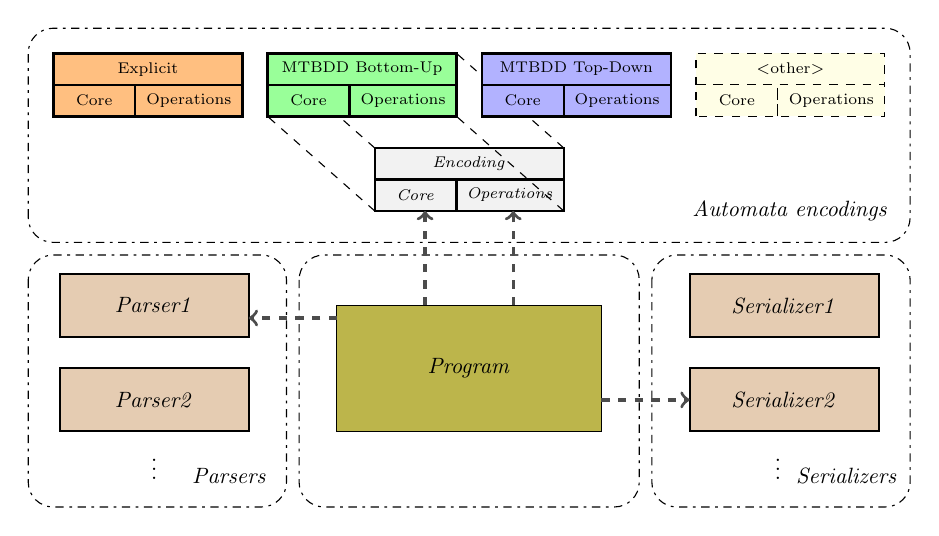
\begin{tikzpicture}
[
  scale=1,
  transform shape,
	gen/.style={thick,fill=gray!10},
	expl/.style={thick,fill=orange!50},
	bu/.style={thick,fill=green!40},
	td/.style={thick,fill=blue!30},
	other/.style={fill=yellow!10,dashed}
]

% encodings
\draw[dashed] (0,1) -- (-1.7,2.5);
\draw[dashed] (0,0) -- (-1.7,1.5);
\draw[dashed] (3,1) -- (1.3,2.5);

\draw (0,0.5) rectangle +(3, 0.5) [gen] node[midway] {\textit{\scriptsize{Encoding}}};
\draw (0,0) rectangle +(1.3, 0.5) [gen] node[midway] {\textit{\scriptsize{Core}}};
\draw (1.3,0) rectangle +(1.7, 0.5) [gen] node[midway] {\textit{\scriptsize{Operations}}};

\draw (-5.1,2) rectangle +(3, 0.5) [expl] node[midway] {\scriptsize{Explicit}};
\draw (-5.1,1.5) rectangle +(1.3, 0.5) [expl] node[midway] {\scriptsize{Core}};
\draw (-3.8,1.5) rectangle +(1.7, 0.5) [expl] node[midway] {\scriptsize{Operations}};

\draw (-1.7,2) rectangle +(3, 0.5) [bu] node[midway] {\scriptsize{MTBDD Bottom-Up}};
\draw (-1.7,1.5) rectangle +(1.3, 0.5) [bu] node[midway] {\scriptsize{Core}};
\draw (-0.4,1.5) rectangle +(1.7, 0.5) [bu] node[midway] {\scriptsize{Operations}};

\draw (1.7,2) rectangle +(3, 0.5) [td] node[midway] {\scriptsize{MTBDD Top-Down}};
\draw (1.7,1.5) rectangle +(1.3, 0.5) [td] node[midway] {\scriptsize{Core}};
\draw (3.0,1.5) rectangle +(1.7, 0.5) [td] node[midway] {\scriptsize{Operations}};

\draw (5.1,2) rectangle +(3, 0.5) [other] node[midway] {\scriptsize{$<$other$>$}};
\draw (5.1,1.5) rectangle +(1.3, 0.5) [other] node[midway] {\scriptsize{Core}};
\draw (6.4,1.5) rectangle +(1.7, 0.5) [other] node[midway] {\scriptsize{Operations}};

\draw[dashed] (3,0) -- (1.3,1.5);

\draw[rounded corners=9,dash pattern=on 3pt off 2pt on 1pt off 2pt] (-5.5,-0.5) rectangle +(14,3.4);

\draw (6.6,0) node {\textit{Automata encodings}};


% parsers
\draw (-5,-2) rectangle +(3, 1) [gen,fill=brown!40] node[midway] (parser1) {\textit{Parser1}};
\draw (-5,-3.5) rectangle +(3, 1) [gen,fill=brown!40] node[midway] {\textit{Parser2}};
\draw (-3.5,-4) node {$\vdots$};

\draw[rounded corners=9,dash pattern=on 3pt off 2pt on 1pt off 2pt] (-5.5,-0.7) rectangle +(4.1,-4);
\draw (-2.3,-4.2) node {\textit{Parsers}};

% serializers
\draw (5,-2) rectangle +(3, 1) [gen,fill=brown!40] node[midway] {\textit{Serializer1}};
\draw (5,-3.5) rectangle +(3, 1) [gen,fill=brown!40] node[midway] {\textit{Serializer2}};
\draw (6.4,-4) node {$\vdots$};

\draw[rounded corners=9,dash pattern=on 3pt off 2pt on 1pt off 2pt] (4.4,-0.7) rectangle +(4.1,-4);
\draw (7.5,-4.2) node {\textit{Serializers}};

% program
\draw[rounded corners=9,dash pattern=on 3pt off 2pt on 1pt off 2pt] (-1.2,-0.7) rectangle +(5.4,-4);

\draw[fill=olive!60] (-0.6,-1.5) rectangle (3.6,-3.5) node[midway] {\textit{Program}};

\draw[very thick,dashed,->,black!70] (-0.6,-1.7) -- (-2,-1.7);
\draw[very thick,dashed,->,black!70] (3.6,-3) -- (5,-3);
\draw[very thick,dashed,->,black!70] (0.8,-1.5) -- (0.8,0);
\draw[very thick,dashed,->,black!70] (2.2,-1.5) -- (2.2,0);

\end{tikzpicture}

		\caption{The main concept of \vata. Figure is taken from \cite{libvata}}.
		\label{fig:vata}
\end{center}
\end{figure}

A \emph{program} (e.g. cli of VATA) employing the three parts of \vata\ works as follows.
An input automaton is loaded by one of the parsers to an intermediate representation.
The wrapping program chooses internal encoding of NTA to which is automaton stored from intermediate encoding (note that it is also
possible to create automaton in the chosen encoding directly using API provided by VATA).
Then the automaton is processed by applying the operations implemented by module of the chosen encoding.
Finally, automaton could be serialized to an output format.
When one wants to add her own encoding then she needs to implement only core of encoding (with API for creating automaton itself)
and needed operations over TA and can employ already implemented parses and serializers in \vata.

\subsection{Implemented NTA Encodings}

It was mentioned that there are currently implemented two representation of TA and both are described in the following subsection.

Using \emph{explicit encoding} NTA transition relation is represented by a hierarchy of the hash tables as it is shown in Figure \ref{fig:explnta}.
The first level of the hash tables hierarchy (\emph{top-level look-up tables}) maps each state $q$ of an automaton to 
a second level of the hash tables hierarchy (\emph{transition cluster}) where are stored all symbols which
are presented in the transition where $q$ is at left-handed side.
Each symbol $a$ in a transition cluster is mapped to a pointer to a set in the third level of hierarchy (\emph{sets of pointers to tuples}).
The set contains pointers to tuples which are at right-handed side in a transition with $q$ at left-handed side and with $a$ as a symbol.
The tuples are stored at a special set where every tuples is stored only once.
Note that it also possible to share part of transition relation between different automata what
brings higher efficiency in space complexity of implementation.
Module for explicit encoding also stores explicitly a set of the final states of a NFA but on
the other side it does not explicitly store a set of all states because it can be obtained from the transition relation.

\begin{figure}[bt]
\begin{center}
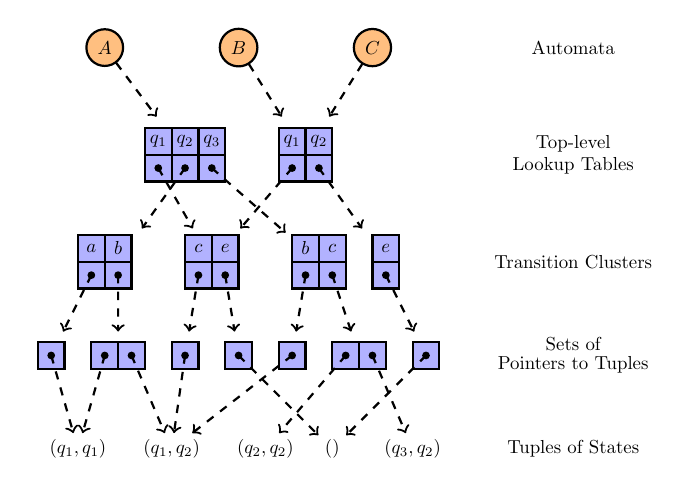
\begin{tikzpicture}
[
  scale=0.85,
  transform shape,
	gen/.style={thick,fill=gray!10},
	expl/.style={thick,fill=orange!50},
	bu/.style={thick,fill=green!40},
	td/.style={thick,fill=blue!30},
	other/.style={fill=yellow!10,dashed}
]

\node at(10,2) {Automata};

\node[expl,circle,draw] (aA) at(1.25,2) {\textit{$A$}};
\node[expl,circle,draw] (aB) at(3.75,2) {\textit{$B$}};
\node[expl,circle,draw] (aC) at(6.25,2) {\textit{$C$}};


\node at(10,0) {\shortstack{Top-level\\ Lookup Tables}};

\node[minimum size=40pt](table1) at (2.75,0) {};
\draw (2,0) rectangle +(0.5, .5) [td] node[midway] {\textit{$q_1$}};
\draw (2,-.5) rectangle +(0.5, .5) [td] node[midway] {};
\draw (2.5,0) rectangle +(0.5, .5) [td] node[midway] {\textit{$q_2$}};
\draw (2.5,-.5) rectangle +(0.5, .5) [td] node[midway] {};
\draw (3,0) rectangle +(0.5, .5) [td] node[midway] {\textit{$q_3$}};
\draw (3,-.5) rectangle +(0.5, .5) [td] node[midway] {};

\node[minimum size=40pt](table2) at (5,0) {};
\draw (4.5,0) rectangle +(0.5, .5) [td] node[midway] {\textit{$q_1$}};
\draw (4.5,-.5) rectangle +(0.5, .5) [td] node[midway] {};
\draw (5,0) rectangle +(0.5, .5) [td] node[midway] {\textit{$q_2$}};
\draw (5,-.5) rectangle +(0.5, .5) [td] node[midway] {};


\draw[->,thick,dashed] (aA) -- (table1);
\draw[->,thick,dashed] (aB) -- (table2);
\draw[->,thick,dashed] (aC) -- (table2);


\node at(10,-2) {Transition Clusters};

\node[minimum size=35](cluster1) at (1.5,-2) {};
\draw (0.75,-2) rectangle +(0.5, .5) [td] node[midway] {\textit{$a$}};
\draw (0.75,-2.5) rectangle +(0.5, .5) [td] node[midway] {};
\draw (1.25,-2) rectangle +(0.5, .5) [td] node[midway] {\textit{$b$}};
\draw (1.25,-2.5) rectangle +(0.5, .5) [td] node[midway] {};

\node[minimum size=35pt](cluster2) at (3.25,-2) {};
\draw (2.75,-2) rectangle +(0.5, .5) [td] node[midway] {\textit{$c$}};
\draw (2.75,-2.5) rectangle +(0.5, .5) [td] node[midway] {};
\draw (3.25,-2) rectangle +(0.5, .5) [td] node[midway] {\textit{$e$}};
\draw (3.25,-2.5) rectangle +(0.5, .5) [td] node[midway] {};

\node[minimum size=35pt](cluster3) at (5.25,-2) {};
\draw (4.75,-2) rectangle +(0.5, .5) [td] node[midway] {\textit{$b$}};
\draw (4.75,-2.5) rectangle +(0.5, .5) [td] node[midway] {};
\draw (5.25,-2) rectangle +(0.5, .5) [td] node[midway] {\textit{$c$}};
\draw (5.25,-2.5) rectangle +(0.5, .5) [td] node[midway] {};

\node[minimum size=35pt](cluster4) at (6.5,-2) {};
\draw (6.25,-2) rectangle +(0.5, .5) [td] node[midway] {\textit{$e$}};
\draw (6.25,-2.5) rectangle +(0.5, .5) [td] node[midway] {};


\draw[thick,fill=black] (2.25,-0.25) circle (0.5mm);
\draw[->,thick,dashed] (2.25,-.25) -- (cluster2);

\draw[thick,fill=black] (2.75,-0.25) circle (0.5mm);
\draw[->,thick,dashed] (2.75,-.25) -- (cluster1);

\draw[thick,fill=black] (3.25,-0.25) circle (0.5mm);
\draw[->,thick,dashed] (3.25,-.25) -- (cluster3);

\draw[thick,fill=black] (4.75,-0.25) circle (0.5mm);
\draw[->,thick,dashed] (4.75,-.25) -- (cluster2);

\draw[thick,fill=black] (5.25,-0.25) circle (0.5mm);
\draw[->,thick,dashed] (5.25,-.25) -- (cluster4);


\node at(10,-3.75) {\shortstack{Sets of\\ Pointers to Tuples}};

\node[minimum size=25pt](set1) at (0.25,-3.75) {};
\draw (0,-4) rectangle +(0.5, .5) [td] node[midway] {};

\node[minimum size=25pt](set2) at (1.5,-3.75) {};
\draw (1,-4) rectangle +(0.5, .5) [td] node[midway] {};
\draw (1.5,-4) rectangle +(0.5, .5) [td] node[midway] {};

\node[minimum size=25pt](set3) at (2.75,-3.75) {};
\draw (2.5,-4) rectangle +(0.5, .5) [td] node[midway] {};

\node[minimum size=25pt](set4) at (3.75,-3.75) {};
\draw (3.5,-4) rectangle +(0.5, .5) [td] node[midway] {};

\node[minimum size=25pt](set5) at (4.75,-3.75) {};
\draw (4.5,-4) rectangle +(0.5, .5) [td] node[midway] {};

\node[minimum size=25pt](set6) at (6,-3.75) {};
\draw (5.5,-4) rectangle +(0.5, .5) [td] node[midway] {};
\draw (6,-4) rectangle +(0.5, .5) [td] node[midway] {};

\node[minimum size=25pt](set7) at (7.25,-3.75) {};
\draw (7,-4) rectangle +(0.5, .5) [td] node[midway] {};


\draw[thick,fill=black] (1,-2.25) circle (0.5mm);
\draw[->,thick,dashed] (1,-2.25) -- (set1);

\draw[thick,fill=black] (1.5,-2.25) circle (0.5mm);
\draw[->,thick,dashed] (1.5,-2.25) -- (set2);

\draw[thick,fill=black] (3,-2.25) circle (0.5mm);
\draw[->,thick,dashed] (3,-2.25) -- (set3);

\draw[thick,fill=black] (3.5,-2.25) circle (0.5mm);
\draw[->,thick,dashed] (3.5,-2.25) -- (set4);

\draw[thick,fill=black] (5,-2.25) circle (0.5mm);
\draw[->,thick,dashed] (5,-2.25) -- (set5);

\draw[thick,fill=black] (5.5,-2.25) circle (0.5mm);
\draw[->,thick,dashed] (5.5,-2.25) -- (set6);

\draw[thick,fill=black] (6.5,-2.25) circle (0.5mm);
\draw[->,thick,dashed] (6.5,-2.25) -- (set7);


\node at(10,-5.5) {Tuples of States};

\node(tup1) at (0.75,-5.5) {$(q_1, q_1)$};
\node(tup2) at (2.5,-5.5) {$(q_1, q_2)$};
\node(tup3) at (4.25,-5.5) {$(q_2, q_2)$};
\node(tup4) at (7,-5.5) {$(q_3, q_2)$};
\node(tup5) at (5.5,-5.5) {$()$};

\draw[thick,fill=black] (0.25,-3.75) circle (0.5mm);
\draw[->,thick,dashed] (0.25,-3.75) -- (tup1);

\draw[thick,fill=black] (1.25,-3.75) circle (0.5mm);
\draw[->,thick,dashed] (1.25,-3.75) -- (tup1);

\draw[thick,fill=black] (1.75,-3.75) circle (0.5mm);
\draw[->,thick,dashed] (1.75,-3.75) -- (tup2);

\draw[thick,fill=black] (2.75,-3.75) circle (0.5mm);
\draw[->,thick,dashed] (2.75,-3.75) -- (tup2);

\draw[thick,fill=black] (3.75,-3.75) circle (0.5mm);
\draw[->,thick,dashed] (3.75,-3.75) -- (tup5);

\draw[thick,fill=black] (4.75,-3.75) circle (0.5mm);
\draw[->,thick,dashed] (4.75,-3.75) -- (tup2);

\draw[thick,fill=black] (5.75,-3.75) circle (0.5mm);
\draw[->,thick,dashed] (5.75,-3.75) -- (tup3);

\draw[thick,fill=black] (6.25,-3.75) circle (0.5mm);
\draw[->,thick,dashed] (6.25,-3.75) -- (tup4);

\draw[thick,fill=black] (7.25,-3.75) circle (0.5mm);
\draw[->,thick,dashed] (7.25,-3.75) -- (tup5);


\end{tikzpicture}

	\caption{Explicit representation of NTA in \vata. Figure is taken from \cite{libvata}}.
	\label{fig:explnta}
\end{center}
\end{figure}

\begingroup
\tikzset{every picture/.style={scale=0.8}}%
\begin{figure}[bt]
	\centering
	\begin{subfigure}{.5\textwidth}
		\centering
		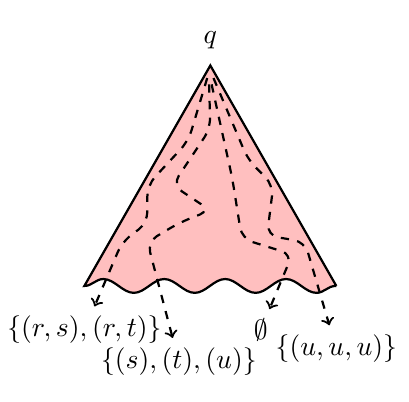
\begin{tikzpicture}
[]
\useasboundingbox (-2.9,-4.9) rectangle (2.7,0.6);

<<<<<<< HEAD
=======

>>>>>>> fcad047018e021c44f6be41eab656d5ec3da0ca5
%\draw[thick,fill=blue!40] (3,-5) -- (0,0) -- (-3,-5) .. controls (-1,-3.5) and (1,-6.5) .. (3,-5);
\draw[thick,fill=pink] (2,-3.5) -- (0,0) -- (-2,-3.5) decorate[decoration=snake,segment length=22] { -- cycle};

\node at (0,0.4){$q$};

\node(set1) at (-2,-4.2) {$\{(r,s),(r, t)\}$};
\node(set2) at (-0.5,-4.7) {$\{(s), (t), (u)\}$};
\node(set3) at (0.8,-4.2) {$\emptyset$};
\node(set4) at (2,-4.5) {$\{(u, u, u)\}$};

\draw[->,thick,dashed,rounded corners] (-0.05,-0.2) -- (-0.35,-1.2) -- (-1,-1.9) -- (-1,-2.5) -- (-1.4,-2.8) -- (set1);
\draw[->,thick,dashed,rounded corners] (-0.02,-0.3) -- (0,-1) -- (-0.6,-1.9) -- (0,-2.3) -- (-0.5,-2.5) -- (-1,-2.8) -- (set2);
\draw[->,thick,dashed,rounded corners] (0.02,-0.3) -- (0.35,-1.8) -- (0.5,-2.75) -- (1.3,-3) -- (set3);
\draw[->,thick,dashed,rounded corners] (0.05,-0.2) -- (0.6,-1.5) -- (1,-1.9) -- (0.9,-2.7) -- (1.5,-2.8) -- (set4);



\end{tikzpicture}
		\caption{MTBDD Top-down representation of a NTA. Image is taken from \cite{libvata}.}
		\label{fig:mtbdd_td}
	\end{subfigure}%
	~
	\begin{subfigure}{.5\textwidth}
	\centering
	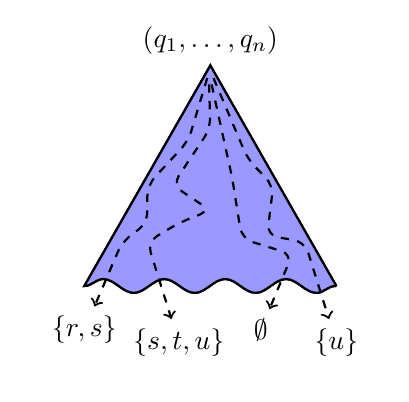
\begin{tikzpicture}
[]
\useasboundingbox (-2.9,-4.9) rectangle (2.7,0.6);
<<<<<<< HEAD
%\draw[thick,fill=blue!40] (3,-5) -- (0,0) -- (-3,-5) .. controls (-1,-3.5) and (1,-6.5) .. (3,-5);
\draw[thick,fill=blue!40] (2,-3.5) -- (0,0) -- (-2,-3.5) decorate[decoration=snake,segment length=22] { -- cycle};

=======

%\draw[thick,fill=blue!40] (3,-5) -- (0,0) -- (-3,-5) .. controls (-1,-3.5) and (1,-6.5) .. (3,-5);
\draw[thick,fill=blue!40] (2,-3.5) -- (0,0) -- (-2,-3.5) decorate[decoration=snake,segment length=22] { -- cycle};


>>>>>>> fcad047018e021c44f6be41eab656d5ec3da0ca5
\node at (0,0.4){$(q_1,\dots, q_n)$};

\node(set1) at (-2,-4.2) {$\{r,s\}$};
\node(set2) at (-0.5,-4.4) {$\{s, t, u\}$};
\node(set3) at (0.8,-4.2) {$\emptyset$};
\node(set4) at (2,-4.4) {$\{u\}$};

\draw[->,thick,dashed,rounded corners] (-0.05,-0.2) -- (-0.35,-1.2) -- (-1,-1.9) -- (-1,-2.5) -- (-1.4,-2.8) -- (set1);
\draw[->,thick,dashed,rounded corners] (-0.02,-0.3) -- (0,-1) -- (-0.6,-1.9) -- (0,-2.3) -- (-0.5,-2.5) -- (-1,-2.8) -- (set2);
\draw[->,thick,dashed,rounded corners] (0.02,-0.3) -- (0.35,-1.8) -- (0.5,-2.75) -- (1.3,-3) -- (set3);
\draw[->,thick,dashed,rounded corners] (0.05,-0.2) -- (0.6,-1.5) -- (1,-1.9) -- (0.9,-2.7) -- (1.5,-2.8) -- (set4);



\end{tikzpicture}
	\caption{MTBDD Bottom-up representation of a NTA. Image is taken from \cite{libvata}.}
	\label{fig:mtbdd_bu}
	\end{subfigure}%
\caption{Semi-symbolic encoding of tree automata.}
\label{fig:symnta}
\end{figure}
\endgroup

Another already implemented encoding is \emph{semi-symbolic} one based on VATA own implementation of MTBDD package.
This encoding is efficient mainly for TA with the large alphabets.
Because semi-symbolic encoding and MTBDD are not in the aim of this thesis they are not be described in detail
but it is possible to find deeper description in \cite{mt:lengal}.
The main principle of semi-symbolic encoding is shown in Figure \ref{fig:symnta}.
First of all it is necessary to distinguish between (a) top-down and (b) bottom-up variants of this encoding.
The first one maps each state $q$ of a NTA using MTBDD to the sets of the tuples of states such that that it is possible
to make transition from $q$ under a symbol $a$ to a tuple in appropriate set (each set of tuples is dedicated
to one symbol under which it is possible to make transition from $q$).
The former one symmetrically maps each n-tuple $(q_1 \cdots q_n)$ of a NFA using MTBDD to the sets of states
where each set $S$ is dedicated to a symbol $a$ of the NFA and contains states such that there exists a transition
with $(q_1 \cdots q_n)$ at the right-handed side and symbol $a$ and state from the set $S$ at the left-handed side.
The final state set of a NTA is again represented by explicit set in both variants,
a state set is not stored explicitly because one can obtain it from the transition relation.
the symbols are encoded (as binary strings) in MTBDD.

All of the mentioned encodings currently support efficient language inclusion checking using algorithm
from \cite{tacas10}.
On the other side the other operations are not currently implemented by all encodings.
The full enumeration of the supported operations for the particular encodings is given in Table \ref{tab:vataop}.

\begin{table}[bt]
	\begin{center}
		\catcode`\-=12
		\begin{tabular}{| l | c | c | c |} \hline
		& {\textbf{Explicit}} & \multicolumn{2}{|c|}{\textbf{Semi-symbolic}} \\ \cline{2-4}
		\textbf{Operation} & \textbf{top-down} & \textbf{bottom-up} & \textbf{top-down} \\ \hline
		Union & $+$ & $+$ & $+$ \\
		Intersection & $+$ & $+$ & $+$ \\
		Complement (experimental) & $+$ & $+$ & $+$ \\
		Removing useless states & $+$ & $+$ & $+$ \\
		Removing unreachable states & $+$ & $+$ & $+$ \\
		Simulation & $+$ & $-$ & $-$ \\
		Downward Inclusion  & $+$ & $+$ & $-$ \\ 
		Upward Inclusion  & $+$ & $-$ & $-$ \\ 
		Simulation over LTS (Labeled Transitions System) & $+$ & $-$ & $-$ \\ \hline
		\end{tabular}
	\caption{Table of supported operations over NTA by particular encodings implemented in \vata.
	Table is taken from \cite{bt:hruska}.}
	\label{tab:vataop}
	\end{center}
\end{table}


\section{Forester}
\label{sec:FA}

Forester is open source tool for verification of program manipulation complex dynamic data structures.
It currently supports program in C language.
Forester is distributed as a \emph{GCC} plugin under GPL license, version 3, and can be obtained from its official website \cite{www:forester}.
Tool is written in C++.

\subsection{Design}

Forester is implemented as a GCC plugin but it does not analyze directly intermediate code of GCC called GIMPLE but it
uses Code Listener infrastructure \cite{cl11} to provide fronted over GIMPLE.

Please see Figure \ref{fig:fa_exec} to get a high level overview of the verification process performed by Forester. 
Forester starts analysis of a program by translation of intermediate code representation provided by Code Listener
to its own microcode.
Microcode represents each program statement by one or few instructions associated abstract transformers.
Symbolic execution is then execute over this microcode.
Abstract domain represented by FA (which are also the core part of a symbolic state) is gradually transformed by the abstract transformers
represented by the microcode instructions during the symbolic execution.
When Forester detects an error the symbolic execution is aborted and the analyzed program is claimed as incorrect one.
When symbolic execution is over then Forester checks whether there is no left garbage (of course, garbage is gradually checked also during the symbolic execution)
and if it is not then a shape invariant has been found and the analyzed program is determined as correct.

\begin{figure}[bt]
	\begin{center}
		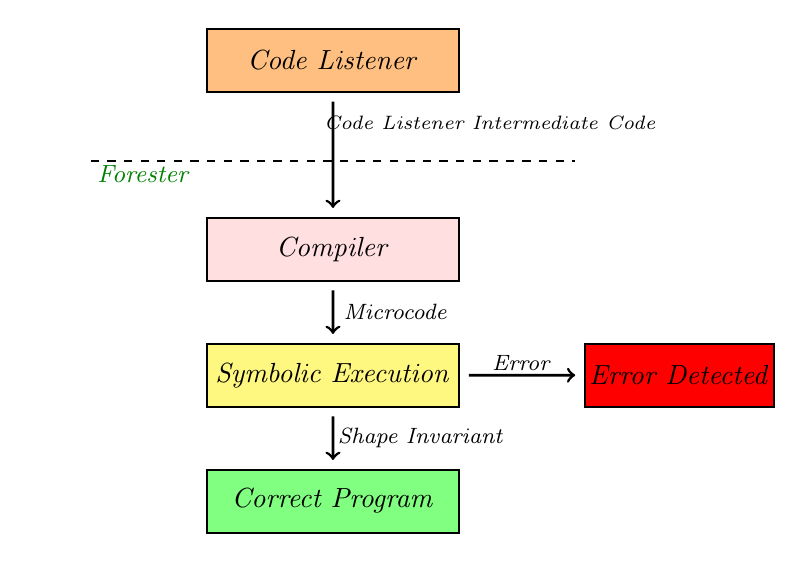
\begin{tikzpicture}[
  cl/.style={thick,fill=orange!50},
  red/.style={thick,fill=Red},
  detection/.style={thick,fill=blue!50},
  compiler/.style={thick,fill=pink!50},
  symexec/.style={thick,fill=yellow!50},
  success/.style={thick,fill=green!50},
  arrow/.style={->,line width=1pt}
  ]

\node (InputNode) at(1.3,10.9) {};
\node (InputDown) at(1.3,10.8) {};

\draw (4,11) rectangle +(4, 1) [cl] node[midway] {\textit{Code Listener}};
\node (CLDown) at(6,11) {};

\draw (4,8) rectangle +(4, 1) [compiler] node[midway] {\textit{Compiler}};
\node (CompUp) at(6,9) {};
\node (CompDown) at(6,8) {};

\draw (4,6) rectangle +(4, 1) [symexec] node[midway] {\textit{Symbolic Execution}};
\node (SymexUp) at(6,7) {};
\node (SymexDown) at(6,6) {};
\node (SymexRight) at(8,6.5) {};

\draw (10,6) rectangle +(3, 1) [red] node[midway] {\textit{Error Detected}};
\node (ErrLeft) at(10,6.5) {};

\draw (4,4) rectangle +(4, 1) [success] node[midway] {\textit{Correct Program}};
\node (CPUp) at(6,5) {};

\draw [arrow] (CLDown) -- (CompUp);
\draw [arrow] (CompDown) -- (SymexUp);
\draw [arrow] (SymexRight) -- (ErrLeft);
\draw [arrow] (SymexDown) -- (CPUp);

\node (LeftFAStart) at(2,9.9) {};
\node (RightFAStart) at(10,9.9) {};
\draw [dashed, line width = 1pt] (LeftFAStart) -- (RightFAStart);

\node (Input) at(8.5,10.5) {\textcolor{Black}{\scriptsize{\textit{Code Listener Intermediate Code}}}};
\node (Input) at(7,7.5) {\textcolor{Black}{\footnotesize{\textit{Microcode}}}};
\node (Input) at(9,6.7) {\textcolor{Black}{\footnotesize{\textit{Error}}}};
\node (Input) at(7.4,5.5) {\textcolor{Black}{\footnotesize{\textit{Shape Invariant}}}};

\node (Input) at(3,9.7) {\textcolor{Green}{\small{\textit{Forester}}}};

\end{tikzpicture}

	\end{center}
	\caption{High level overview of Forester program analysis.}
	\label{fig:fa_exec}
\end{figure}

A little deeper description of conceptual design of Forester (which is shown in Figure \ref{fig:fa_design}) and relations
between its modules is going to be given now.
Please note that implementation of Forester is not explicitly separated to the stand-alone compilation modules so the notion of the modules
used in following text is more abstract to provide reader basic summary of the Forester design.
One module could be e.g. a set of closely related classes with a similar purpose.
As it was mentioned above the Code Listener representation of GCC intermediate code is mainly used by Forester \emph{Compiler} module.
Compiler then converts Code Listener instructions to the Forest own \emph{Microcode Instructions} and creates their list over which the \emph{Symbolic Execution} is performed.
Symbolic execution then execute microcode instructions (abstract transformers) which manipulates \emph{Symbolic State} and of course
also \emph{Forest Automata} included in symbolic states.
Symbolic execution also need \emph{Symbol Context} which is created for each function (and also for global space)
and keeps information about variables used in the function, about function arguments or about stack frame layout.
A symbolic state provides information about the state of the heap which is represented by a FA and it also keeps the information about
the corresponding microcode instructions.
\emph{Forest Automata} module provides methods for manipulation FA need during verification procedure.
The operations like normalization or abstraction over FA are not part of the module containing FA implementation but are provided
like classes which take FA as parameters.
So these operation could be understood as another module \emph{Operation over Forest Automata}.
Finally, Forester currently has its own implementation of \emph{Tree Automata}.
It is very lightweighted implementation containing optimized operations directly for Forester purposes.
One of them is operation for language inclusion checking using simulation which efficiency is also crucial for Forester performance.
The advantage of this implementation is its simplicity and
the efficiency get by optimizing the implementation specially to the Forester.
On the other side, it is not easy to maintain such a optimized implementation.
Especially, when one considers that there is still progress in field of design of the efficient algorithms
and the improvement of an algorithm brings much higher efficiency then implementation optimization.

\begin{figure}[bt]
	\begin{center}
		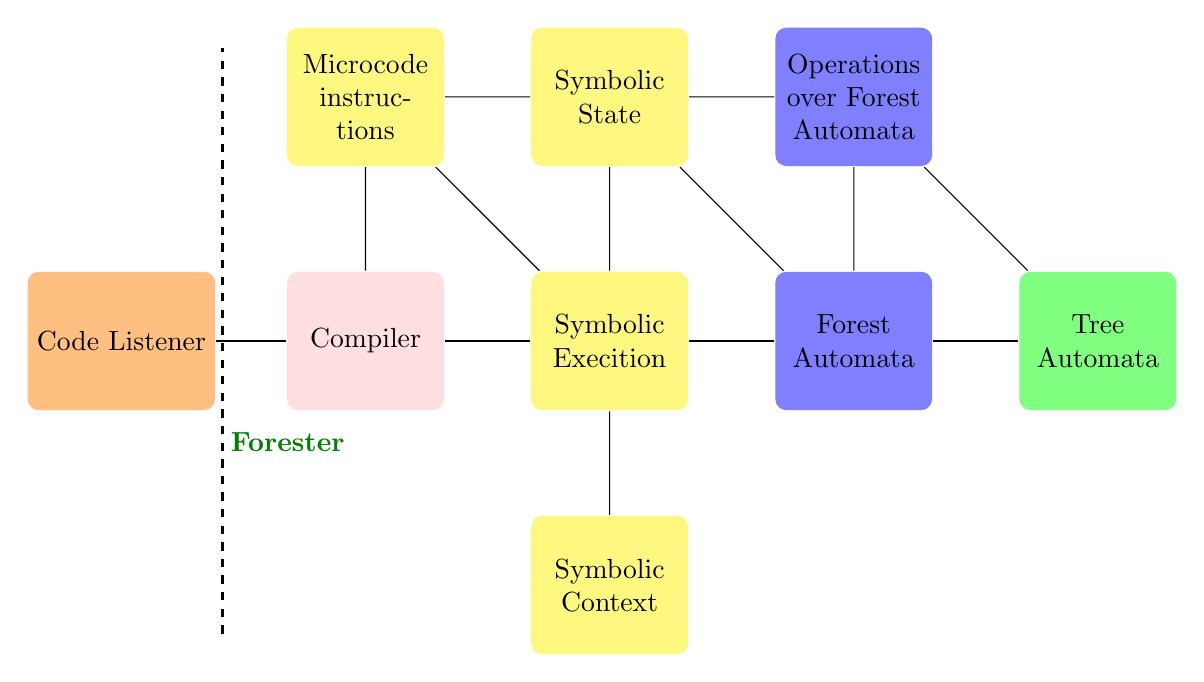
\begin{tikzpicture}[
  scale=0.8,
  node distance = 3.1cm,
  block_cl/.style={rectangle, text centered, rounded corners, thick, fill=orange!50,
    minimum height = 5em, minimum width = 3em},
  block_compiler/.style={rectangle, text centered, rounded corners, thick, fill=pink!50,
    minimum height = 5em, minimum width = 3em, text width = 5em},
  block_symex/.style={rectangle, text centered, rounded corners, thick, fill=yellow!50,
    minimum height = 5em, minimum width = 3em, text width = 5em},
  block_fa/.style={rectangle, text centered, rounded corners, thick, fill=blue!50,
    minimum height = 5em, minimum width = 3em, text width = 5em},
  block_ta/.style={rectangle, text centered, rounded corners, thick, fill=green!50,
    minimum height = 5em, minimum width = 3em, text width = 5em},
  line/.style={draw, -}
  ]

\node [block_cl] (cl) {Code Listener};
\node [block_compiler, right of=cl] (compiler) {Compiler};
\node [block_symex, above of=compiler] (microcode) {Microcode instructions};
\node [block_symex, right of=compiler] (symex) {Symbolic Execition};
\node [block_symex, above of=symex] (symstate) {Symbolic State};
\node [block_symex, below of=symex] (symcnt) {Symbolic Context};

\node [block_fa, right of=symex] (fa) {Forest Automata};
\node [block_fa, above of=fa] (faop) {Operations over Forest Automata};

\node [block_ta, right of=fa] (ta) {Tree Automata};

\path [line] (cl) -- (compiler);
\path [line] (microcode) -- (compiler);
\path [line] (symex) -- (compiler);
\path [line] (symex) -- (symstate);
\path [line] (symex) -- (symcnt);
\path [line] (symex) -- (fa);
\path [line] (symstate) -- (fa);
\path [line] (microcode) -- (symex);
\path [line] (fa) -- (faop);
\path [line] (fa) -- (ta);
\path [line] (symstate) -- (faop);
\path [line] (faop) -- (ta);
\path [line] (microcode) -- (symstate);

\node (LeftFAStart) at(2,-6) {};
\node (RightFAStart) at(2,6) {};
\draw [dashed, line width = 1pt] (LeftFAStart) -- (RightFAStart);
\node (Input) at(3.3,-2) {\textcolor{Green}{\textbf{Forester}}};

\end{tikzpicture}

	\end{center}
	\caption{Conceptual design of Forester.}
	\label{fig:fa_design}
\end{figure}

Please note, this is just the conceptual high level view of Forester design.
A real implementation is much more complicated (e.g. Forest automata are implemented by two classes: \emph{FA} and \emph{FAE})
and full of the technical details.
A full description of the implementation is also not the aim of this text.

It was already mentioned that substitution of Forester TA implementation by
VATA could bring some advantages.
We summarize them here again.
The first one is that it is much easier to maintain one library where
the state-of-the-art algorithms are implemented and optimized.
Since VATA and Forester is developed by the same developers it also easy to added
to VATA operations needed by Forester.
Having narrow interface between TA library and the rest of Forester
also improves code quality of Forester in the sense of modularity, maintainability and code organization.
These arguments lead us to implement a version of Forester using VATA.
This is described in Section \ref{ch:fova}.


\subsection{Implementation of Forest Automata concepts}
\label{subsec:faimpl}

This subsection describes implementation of forest automata based verification procedure in Forester.
The core of forest automata module is class {\tt FA}.
The implementation corresponds to the definitions given in Chapter \ref{ch:prel}.
Class FA has a data member representing vector of tree automata $(t_1 \cdots t_n)$.
It also has a data member keeping a reference to an automaton representing global variables
and a reference to the automata representing variables of current function. %TODO define ABP
The labels of TA are represented by structure {\tt NodeLabel}.
This structure contains a data member determining type of node
(whether it is a general node, a data node or a node containing vector of data).
The structure also has data member that keeps value of type that is stored in label.
The basic operations over FA (like adding or removing a TA from FA) are encapsulated in class FA.
The other class providing operations over FA is {\tt FAE}. 

As it was already mentioned the forest automata are further used in symbolic state.
The implementation of symbolic state is in class {\tt SymState}.
The class keeps reference to a Forester microcode instruction $I$ to which symbolic state corresponds.
It has data member that is a pointer to forest automaton $F$ (instance of class {\tt FAE})
representing actual memory state.
Another data member of class SymState is a set of registers $\regsset$ with data values in the symbolic state.
We denote set $\regsset$ by $\regs$. 
The register can be local or global ones.
The global registers contain the references to the forest automata modelling
the global state of a program what is a forest automata modelling the block of global variables.
The local registers serve as temporary memory used in
the microcode instructions for data manipulation.
Putting together data members of class {\tt SymState}
we can define symbolic state formally as a triple $S=\symstate{F}{\regs}{I}$.
The values of register are instances of a structure {\tt Data}.
The structure consists data members keeping information about type of data $T$, its size $S$,
value $V$ of type $T$ and information about its nested members $MBS$.
We can again fomally define structure Data as $\ddata$ where
$T$ is a data type,
$S \in \natnum$ is size of data,
$V$ is a value of type $T$,
$MB=(D_1 \cdots D_n)$ represents nested data if they are present (this is the case when $D$ represents a data structure)
and $D_i$ is another instance of data.
$T$ could be one of the following data types: pointer, reference to a TA, integer, boolean, structure or some other data type.
$T$ could be also undefined or it could state that type is unknown.
We describe in detail one of types, the root reference whose values are defined as $RR=({\tt Root},{\tt Displ})$
where ${\tt Root} \in \natnum$ is an index of a tree automaton in $F$
and ${\tt Displ} \in \natnum$ is an index of successor of a root pointed by ${\tt Root}$.
The operation for manipulation with symbolic state are partially provided by class {\tt SymState}
and some additional operations are provided by class {\tt VirtualMachine}.

We already described the data structures used for implemetation of forest automata concepts
and related symbolic execution.
The symbolic execution using this data structures is realized by gradually appending
and removing symbolic states from a queue.
When a symbolic state is taken from the queue a microcode instruction contained in
the symbolic state is executed.
Some instructions during its execution appends a new symbolic state to the queue.
Symbolic execution finishes when queue is empty.
The microcode instructions executed during symbolic execution are described in folowing Section \ref{subsec:instrs}

\subsection{The Microcode Instructions}
\label{subsec:microinstr}

This sections provides a description of the Forester microcode instruction
but before describing their semantics itself the notion used further is given first.
We use $r_s \in \regs$ to denote the source register,
$r_d \in \regs$ to denote the destination register,
$r_l \in \regs$ to denote a local register and
$r_g \in \regs$ to denote a global register.
Note that source register is also global or local and same holds for the destination register.
The source and destination registers are parameters of some instructions in the following text.
We use $\regssub{r}{r'}$ to denote a set of registers which has the same values as registers in $\regs$
excluding $r$ that has value $r'$.
A symbol $I_n$ denotes next instruction following an instruction actually executed.
We define semantics of each instruction formally using a function 
$f: \instrset \times \symset \rightarrow \symset$
where $\symset$ is a set of all symbolic states and $\instrset$ is a set of all instructions.
When it is clear for which instruction is used we ommit the first parameter of $f$.
The function $f$ defines an effect of instruction as transformation of current
symbolic state $s$ to a new symbolic state $s'$.

A list of the microcode instructions used in Forester with description
of their semantics follows.
Each instruction is described informally first and then its effect is defined
in the notion of function $f$.
Firstly, the most crucial instructions are described then the complete list is finished.
\begin{itemize}
	\item {\tt FI\_acc\_sel} isolates the $i$-th selector which is a given root of TA.
		The root of TA is defined by a destination register.
		This instruction checks whether a selector pointed by the destination register
		selects a node that represents allocated memory node or undefined pointer.
		In the first case the node is isolated to an new TA and the original node in the
		orignal TA is replaced by a root reference to a new TA.
		In the second case nothing changes.
		Note that this basically corresponds to identification of the cut-points
		and their seperation to a new TA.
		
		$f(\stdsym) = \symstate{F'}{\regs}{I_n}$
		where $F'$ is a new FA obtained from $F$ by isolating
		the $i$-th selector of root of TA $t$.
		TA $t$ and correct selector are determined by root reference $RR=(Root, Displ)$
		in the register $r_d$ such that $Root$ points to $t$ and $i=Displ+o$
		where $o$ is a offset which is a parameter of this instruction.

	\item {\tt FI\_acc\_set,FI\_acc\_all} instruction does the same thing as the previous one
		but for a set of selectors or for all selectors of a given root of TA.

	\item {\tt FI\_alloc} instruction creates a new instance of structure {\tt Data} $\ddata$
		that represents allocated memory.
		The size $S$ of $D$ is determined by an integer value in the source register.
		The created instance will be further used for creating of a new TA.
		
		$f(\stdsym) = \symstate{F}{
		\regssub{
			r_{d}}
			{x}}
		{I_n}$
		where $x=({\tt void\_ptr},{\tt undef},S',\emptyset)$ is an instance of structure Data
		such that $S'$ is a size stored in $r_s$ (where should be stored an integer value). 
	
	\item {\tt FI\_node\_create} instructions creates a new node
		(and hereby also a new TA) which is a root node of the new TA.
		A reference to the new TA is stored to destination register.
		A type info of the new node and its size is obtained from source
		register.
		
		$f(\stdsym) = \symstate{F'}{
		\regssub{
			r_{d}}
			x}
		{I_n}$
		where $F'$ is a new FA created by adding newly created TA $t$ to $F$
		and $x$ is a reference to $t$.
		TA $t$ has selectors defined in $r_s$. 
		Note that reference to $t$ is not added to a TA in $F$ in this step
		but it is done by instruction assigning a register value to a
		node of TA.
	
	\item {\tt FI\_node\_free} instruction deletes a node in FA and
		invalidate all references to it.
		
		$f(\stdsym) = \symstate{F'}
		{\regs}
		{I_n}$
		where $F'$ is obtained from $F$ by deleting a TA $t$ referenced
		by a value of $r_s$ and removing all reference to $t$ from TA of $F$.

	\item {\tt FI\_abs, FI\_fix} instructions computes fixpoint with (FI\_abs) or
		without ({\tt FI\_fix}) abstraction.
		
		$f(\stdsym) = \symstate{F'}
		{\regs}
		{I_n}$
		where $F'$ is a new FA obtained from $F$ by computing fixpoint with or without abstraction.

\end{itemize}

Since we already covere the most crucial instructions we describe
the rest of the instructions now.
The following instructions are used for manipulating registers.

\begin{itemize}

	\item {\tt FI\_load\_cst} instruction loads a constant to a register.
		So it creates a new symbolic state which differs only in register content.
		
		$f(\stdsym) = \symstate{F}{\regssub{r_d}{c}}{I_n})$ where
		$c$ is a constant which is parameter of this instruction.
	
	\item {\tt FI\_move\_reg} instructions creates a new symbolic state where
		a value from $r_s$ is moved to register $r_d$.
		
		$f(\stdsym) = \symstate{F}{\regssub{r_d}{r_s}}{I_n}$.
	
	\item {\tt FI\_bnot, FI\_inot} instructions negate a value in a register and
		creates a new symbolic state with the negated value in the register.
		{\tt FI\_bnot} negates integer and {\tt FI\_inot} negates boolean value.
		
		$f(\stdsym) = \symstate{F}{\regssub{r_d}{\neg r_d}}{I_n}$.
	
	\item {\tt FI\_move\_reg\_offs} instruction accesses a tree automaton pointed
		by a reference in a source register and increases its {\tt displacement} value by a given offset.
		The new value is stored a destination register.
		
		$f(\stdsym) = \symstate{F}{\regssub{r_d}{\rreftuple{\droot}{\ddispl+o}}}{I_n}$
		where $o$ is offset which is parameter of this instruction
		and $\rrefreg{r_s}$.
	
	\item {\tt FI\_move\_reg\_inc} instruction does same thing as the previous one but
		it increases a displacement by a value in the second source register (which is
		present for this instruction).
		
		$f(\stdsym) = \symstate{F}{\regssub{r_d}{\rreftuple{\droot}{\ddispl + r_{s_2}}}}{I_n}$
		where $r_{s_1} \in \regs, r_{s_2} \in \regs$ are source registers such that
		$\rrefreg{r_{s_1}}$, $r_{s_2}$ has integer value.
	
	\item {\tt FI\_get\_greg} loads a value from a global register to
		a local register.
		
		$f(\stdsym) = \symstate{F}{\regssub{r_{ld}}{r_{gs}}}{I_n}$.
	
	\item {\tt FI\_set\_greg} loads a value from a local register to
		a global register.
		
		$f(\stdsym) = \symstate{F}{\regssub{r_{gd}}{r_{ls}}}{I_n}$.
	
	\item {\tt FI\_get\_ABP} loads a root reference to a FA representing
		a memory pointed by local variables and adds an offset to a displacement
		in the root reference.
		
		$f(\stdsym) = \symstate{F}{\regssub{r_d}{
			\rreftuple{\droot}{\ddispl + o}}}
			{I_n}$ where $\rrefreg{r_{ABP}}$ is the register containing root
		reference to FA representing local memory and $o$ is offset
		which is parameter of this function.
	
	\item {\tt FI\_get\_GLOB} loads a root reference to a FA representing
		a memory of local function to a local register
		and adds an offset to a displacement in the root reference.
		
		$f(\stdsym) = \symstate{F}
			{\regssub{r_{d}}{
				\rreftuple{\droot}{\ddispl + o}
			}}
			{I_n}$ where $\rrefreg{r_{GLOB}}$ is the register containing root
			reference to FA representing global memory and $o$ is offset
			which is a parameter of this instruction.
	
	\item {\tt FI\_load} loads a value from a FA pointed
		by a root reference in source register to a destination register.
		The value is value of the $i$-th successor of the root pointed
		by source register value, where $i$ is a value of offset.
		
		$f(\stdsym) = \symstate{F}
			{\regssub{r_{d}}{
				\rreftuple{\droot}{\ddispl + o}
			}}
			{I_n}$
			where $\rrefreg{r_{s}}$,
			$F[i]$ is a TA of F,
			$o$ is offset which is a parameter of this instruction,
			$i=\droot$,
			$displ=\ddispl + o$.
	
	\item {\tt FI\_load\_ABP, FI\_load\_GLOB} same as the previous instruction
		but loads a value from a FA pointed by $r_{ABP}$ or $r_{GLOB}$ register.
		
		Fomally it could be defined as the previous instruction but
		$r_{ABP}$ and $r_{GLOB}$ are used instead of $r_s$.
	
	\item {\tt FI\_store} instruction stores a value from source register
		to a TA pointed by destination register.
		The location is the $i$-th successor of a root of the FA where $i$ is offset
		obtained as a parameter of this instruction.
		
		$f(\stdsym) = \symstate{F'}{\regs}{I_n}$
		where $F'$ is a FA obtained from $F$ by assignemnt
		$S_{F[i]}^{displ} = r_{d}$,
		$F[i]$ is a TA of $F$ referenced by root reference $\rref$ stored in $r_s$ register,
		$o$ is offset which is a parameter of this instruction,
		$i=\droot$ and $displ=\ddispl + o$.
	
	\item {\tt FI\_loads, FI\_stores} instructions do same as the previous
		one but manipulates the structures.
		
		Formal definition is also same but result in the register $r_d$ (in case of {\tt FI\_loads})
		and or in the corresponding (in case of {\tt FI\_stores}) has a different typed
		(concretely it is a structure).

	\item {\tt FI\_push\_greg} instruction creates a new global register
		and fills it with a value in a source register.
		
		$f(\stdsym) = \symstate{F}
		{\regs\cup \{r_g\}}
		{I_n}$
		where $r_g$ is a new global register such that $r_g = r_s$.
	
	\item {\tt FI\_pop\_greg} instruction takes a value in the last created
		global register and stores it to a local register.
		The global register is then deleted.
		
		$f(\stdsym) = \symstate{F}
		{\regssubmin{r_g}{r_d}{r_g}}
		{I_n}$
		where $r_g$ is the lastly created global register.

	\end{itemize}

	Finally, the remaining instructions do not perform a specific operations
	but perform the various operations like conditions, arithmetic operations or
	aborting the symbolic execution, etc.

	\begin{itemize}

	\item {\tt FI\_cond} instruction represents condition in original code.
		It creates a new symbolic state with same forest automaton and appends
		it to the queue.
		The new state contains an instruction which corresponds to a \textit{then}
		or \textit{else} branch of the condition.
		The instruction for the new state is chosen according to
		the content of {\tt FI\_cond} instruction symbolic state register.
		
		$f(\stdsym) = \symstate{F}{\regs}{r_s ? I_t : I_f}$
		where $I_t$ is instruction used when $r_s$ has true value and
		$I_f$ is instruction used otherwise.


	\item {\tt FI\_iadd, FI\_imull} instructions performs integer
		addition and multiplication.
		
		$f(\stdsym) = \symstate{F}
		{\regssub{r_d}{r_{s_1} \otimes r_{s_2}}}
		{I_n}$
		where $r_{s1} \in \regs, r_{s2} \in \regs$, $\otimes \in \{+,*\}$
		are two source registers with values of integer type.

	\item {\tt FI\_eq, FI\_neq, FI\_ge, FI\_gt, FI\_le, FI\_lt} instructions
		makes a comparison corresponding to their names.
		The result of the comparison stores to a destination register.
		
		$f(\stdsym) = \symstate{F}
		{\regssub{r_d}{r_{s_1} \otimes r_{s_2}}}
		{I_n}$
		where $r_{s_1} \in \regs, r_{s_2} \in \regs$ are two source registers
		and $\otimes \in \{=,\neq, <,>,\leq,\geq\}$.
	
	\item {\tt FI\_build\_struct} instruction creates a structure from a
		content of registers and result stores to a destination register.
		The source registers are defined by an index of the first register and
		vector of offsets from this register which points to another registers
		that are used for creating structure.
		
		$f(\stdsym) = \symstate{F}
		{\regssub{r_d}{x}}
		{I_n}$
		where $x$ is a structure created from values of registers $r_s,r_{s+i_1},r_{s+i_2}, \ldots, r_{s+i_n}$.
		The values $i_1, i_2, \ldots, i_n$ are offsets defined as parameters of this instruction.

	\item {\tt FI\_check} instruction checks whether there is not
		garbage.
		
		$f(\stdsym) = \symstate{F'}
		{\regs}
		{I_n}$
		where $F'$ is obtained from $F$ by removing all unreachable
		TA.
	
	\item {\tt FI\_abort} instruction aborts program execution.
	
	\item {\tt FI\_assert} instruction checks whether a value
		in a givem register is the same one as a constant.
		
		$f(\stdsym) = \stdsym$ if $r_s = c$, otherwise
		symbolic execution is aborted.
		Constant $c$ is a parameter of this instruction.
	
	\item {\tt FI\_error} instruction throws an exception representing
		a local error in program.
	
	\item {\tt FI\_noret} instruction quits program symbolic execution when
		no return function end is reached.

\end{itemize}

\bexmp
	We illustrate how a program in C is represented by the described instructions.
	Consider the following C program.

	\begin{quote}
	\begin{verbatim}
	1: struct T {
	2:    struct T* next;
	3: };

	4: int main()
	5: {
	6:    struct T* x;

	7:    x = (struct T*) malloc(sizeof(struct T));
	8:    free(x);

	9:    return 0;
	10:}
	\end{verbatim}
	\end{quote}

	Now we present a microcode instructions to which the statement at the line $7$ is translated.
	\begin{quote}
	\begin{verbatim}
	1: mov r0, (int)4
	2: alloc r0, r0
	3: node r0, r0, next[0:4:+0]
	4: mov r1, ABP + 0
	5: mov [r1 + 12], r0    
	6: check
	\end{verbatim}
	\end{quote}

	Firstly the size of a new allocated (in this case size is $4$) data is stored to register $r_0$ at line $1$.
	Then the new instance of structure {\tt Data} $D$ is created and stored to $r_0$ at line $2$.
	A new TA $t$ is created at line $3$.
	The TA $t$ has one transition from the root with label that consists one pointer selector {\tt next} whose
	displacement in label is $0$ and size is $4$.
	A root reference to $t$ is stored to $r_0$.
	Finally lines $5$ a $6$ performs adding root reference pointing to $t$ is added to a TA that represents
	a memory state of the actually executed function (which is in this case {\tt main}).
\eexmp

\chapter{Forester with VATA}
\label{ch:fova}

This chapter describes a process of porting Forester to \vata, its difficulties and design and it also deals with implementation
itself.

First of all it is important to declare that we use \vata\ implementation of explicit encoding of TA because
it is currently the only one that support the most of needed operations over TA and it is also more efficient than
semi-symbolic encoding for purposes of Forester because no large alphabets are used during the verification procedure
so the advantage of the semi-symbolic encoding would not be fully utilized here.

Forester implementation is currently far from being mature and high structural dependency is
one of its bottlenecks.
So the first thing needed to be done is reducing number of dependencies between classes (described in Section \ref{sec:forester_prep}).
Then it would be possible to apply design pattern \emph{adapter} \cite{gamma95} (described in Section \ref{sec:adapter}) to create
an interface between Forester and \vata\ (implementation itself is described in \ref{sec:fova_impl}).
Applying of adapter design pattern makes possible to include VATA without need of rewriting
Forester to the names of methods and data used in VATA.
It creates also only one place (particularly adapter class) connecting Forester and VATA instead of
including VATA into many of the Forester classes and so it prevents from creating too strong relation between them.

\section{Forester Refactoring}
\label{sec:forester_prep}

The original implementation of tree automata library has also strong dependencies
the other classes.
Hence it was needed to refactore implementation before it was possible to create adapter class for VATA API.
The core class of original tree automata is class \emph{TA} and there are also related classes,
e.g. class \emph{TT} for transitions representation or class \emph{Antichain} for language inclusion checking using the Antichain algorithm from \cite{tacas10}.
This set of classes realizing original tree automata library will be further referred as \emph{tree automata module}.

The refactoring is mainly based on reduction of a number of data types and data members declared
to be \emph{public} (in sense of the C++ programming language).
This is by exploiting features provided by C++11 \cite{stroustrup13} which brings methods (keyword \emph{auto})
for auto deduction of the data types by compiler.
That provides possibility to make some of data types of the original tree automata module \emph{private}.
\emph{Iterator} is another concept often used in combination with auto deduction of types to reduce the need to export internals of tree automata module.
The combination of these two patterns are used for example when one needs to iterate over all transitions of tree automata or all transitions which
have same state as parent.
These kinds of iterations are quite common in Forester.
Another part of refactoring consists of simple replacing access of the class data members by the corresponding getters and setters method.
Reducing of structural dependencies is also done by emphasis application of \emph{Law of Demeter} \cite{lod89} what practically
means that classes using TA explicitly should implement methods providing information about TA instead of providing object representing TA itself.
E.g., when one class wants to know whether a given state is final in an tree automaton of an forest automaton then FA implementation should
implement a method providing this information instead of providing access to its TA.
Applying the Law of Demeter reduces knowledge needed about implementation of TA module across the whole project.
That helps us to make a smaller interface for TA module.
However, also after this refactoring Forester source code is still far from accomplishing the mentioned good practices (and also those not mentioned)
in the whole source code.

\section{Adapter Design Pattern}
\label{sec:adapter}

\emph{Adapter} is structural design patter \cite{gamma95} used for creating interface between classes incompatible classes.
Adapter in notion of UML is shown in Figure \ref{fig:adapter}.
Adapter consists from a class \emph{Adaptee} which is the class that we want to make compatible with
another class \emph{Client} which wants to use the methods of Adaptee.
Class \emph{Adaptor} is the one providing connection between Client and Adaptee.
Adaptor could be implemented as inherited class from Adaptee and employs the concept of inheritance to redirect
method calls to its parent (with some possible preprocessing).
Another possible implementation is composing Adaptee to Adaptor and using Adaptor like an interface to Adaptee.
Adaptor also could add a new method that combines Adaptee methods to achieve wanted operations.

\begin{figure}
	\begin{center}
		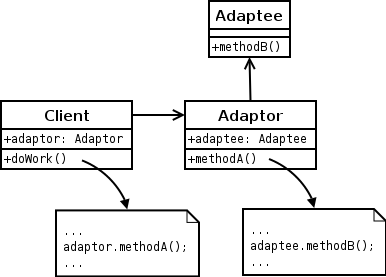
\includegraphics[scale=0.5]{fig/adapter.png}
	\end{center}
	\caption{Adapter design pattern expressed in UML.
	Picture is taken from \cite{wiki:adapter}}.
	\label{fig:adapter}
\end{figure}

Let us show what the mentioned roles are in our case.
Adaptee is the API of \vata, specifically it is the class \emph{ExplicitTreeAut} implementing representation of a tree automaton in explicit encoding.
Client is in our case not just one class but it is a set of the Forester classes using TA library.
Adaptor is a newly implemented class \emph{VATAAdapter} which description is in the following section.

\section{Implementation}
\label{sec:fova_impl}

The main part of the adapter patter is in our case newly implemented class \emph{VATAAdapter} playing role of Adaptor.
We decided to used the implementation approach to Adaptor, preferring composition over inheritance,
because it is more suitable for our purposes since we often needs to rename methods 
(name of a method in Forester differs from name of a method in VATA performing same operation)
or conversion of parameters data type (e.g. from vector to set). 

The class \emph{VATAAdapter} instantiates class \emph{ExplicitTreeAut} from VATA as its private data member
and redirects to this instance method calls from Forester (the names of methods of VATAAdapter are the same as they were
in the original TA library).
\emph{VATAAdapter} also sometimes performs mentioned conversion of the data types.
There are methods implemented by adapter not presented in VATA like method \emph{unfoldAtRoot}
performing some kind of an unfolding.
The methods of this kind are very Forester specific so it is not sensible to add them to general purpose library like VATA is.

We originally supposed that it would be possible to keep the original TA module along VATA adapter
to be able to easily switch between them.
However it has proved that this would bring high overhead in some situations.
A conversion of some data types is needed compared to situation when there are used directly data types compatible with VATA in the Forester code.
Hence we decided to remove the original tree automata module and further support only version of Forester with \vata.

\chapter{Backward Run in Forest Automata Based Verification(Text text)}
\label{ch:backward}
text

\section{Backward Run over Symbolic Context}

This sections provides a description of the reverse operations for
each instruction of Forester microcode which were introduced in Section \ref{subsec:microinstr}.
We describe each instruction informally first and then the instruction is defined in notion
of a function $\grev: \grevinter$ which should has reverse semantics to the function $f$ from Section \ref{subsec:microinstr}.
So $\grev$ takes as parameter a symbolic state and an instruction and returns a new symbolic state representing
a symbolic state in the forward symbolic execution right before execution of the instruction.
Note that not all instructions need to be reversed but only those
modifying forest automata or those affecting further modification of forest automata.
All the notion used in the following text is the same as the one defined in Section \ref{subsec:microinstr,subsec:faimpl}.
We present the crucial instructions first then the rest is given.
\begin{itemize}
	\item {\tt FI\_acc\_sel}
		
	\item {\tt FI\_acc\_set,FI\_acc\_all}

	\item {\tt FI\_alloc}

	\item {\tt FI\_node\_create}
	
	\item {\tt FI\_node\_free}

	\item {\tt FI\_abs, FI\_fix}

\end{itemize}

Since we already covere the most crucial instructions we describe
the rest of the instructions now.
The following instructions are used for manipulating registers.

\begin{itemize}

	\item {\tt FI\_load\_cst}

	\item {\tt FI\_move\_reg}

	\item {\tt FI\_bnot, FI\_inot}

	\item {\tt FI\_move\_reg\_offs}

	\item {\tt FI\_move\_reg\_inc}

	\item {\tt FI\_get\_greg}

	\item {\tt FI\_set\_greg}

	\item {\tt FI\_get\_ABP}

	\item {\tt FI\_get\_GLOB}

	\item {\tt FI\_load}
	
	\item {\tt FI\_load\_ABP, FI\_load\_GLOB}
	
	\item {\tt FI\_store}

	\item {\tt FI\_loads, FI\_stores}

	\item {\tt FI\_push\_greg}
	
	\item {\tt FI\_pop\_greg}

	\end{itemize}

	Finally, the remaining instructions do not perform a specific operations
	but perform the various operations like conditions, arithmetic operations or
	aborting the symbolic execution, etc.

	\begin{itemize}

	\item {\tt FI\_cond}

	\item {\tt FI\_iadd, FI\_imull}

	\item {\tt FI\_eq, FI\_neq, FI\_ge, FI\_gt, FI\_le, FI\_lt}
	
	\item {\tt FI\_build\_struct}

	\item {\tt FI\_check}

	\item {\tt FI\_abort}
	
	\item {\tt FI\_assert}

	\item {\tt FI\_error}

	\item {\tt FI\_noret}

\end{itemize}


\section{Intersection of Forest Automata}

\chapter{template$<$class Text$>$ Implementation(Text text)}
\label{ch:impl}
text

\section{Execution Trace}
\section{Module For Intersection}

\chapter{template$<$class Text$>$ Evaluation(Text text)}
\label{ch:eval}
text

\chapter{Conclusion}
\label{ch:concl}

The main goals of this thesis were (a) to implement version of Forester tool that uses the VATA library for tree automata representation and manipulation
and (b) to extend verification procedure based on forest automata with backward run for detection of the spurious errors found in the analysed program.
The theory of forest automata and related theory of tree automata has been studied and described in this thesis and the verification procedure
based on forest automata has been also explored to fulfill the thesis goals.
The connection of Forester and \vata\ was designed and implemented after the analysis of the both tools.
Forester had to be refactored for this purposes.

The first goal has been already reached and the version of Forester using the VATA library successfully participated in competition SV-COMP 2015 \cite{www:svcomp}.
The knowledge about Forester and related verification procedure gained during the work on the term project will be further employed for design
and implementation of backward run in the Forester tool which is the second goal of this master thesis.

